% !TEX root = ../MasterThesis_goto_v1.tex

%%%%%%%%%%%%%%%%%%%%%%%%%%%%%%%%%%%%%%%%%%%%%%%%%%%%%%%%%%%%%%%%%%%%%%%%%%%%%%%%%%%%%%%%%%%%%%%%%%%%%
\chapter{深層学習を用いた崩壊点検出} \label{chap:VertexFinderwithDL}

本章では, 深層学習を用いた崩壊点検出について述べる。
前章では崩壊点検出のためのネットワークとして, 「1. 飛跡対についてのネットワーク」, 「2. 任意の数の飛跡についてのネットワーク」の二つのネットワークを導入した。
しかし, これら個々のネットワーク単体では崩壊点検出を実現できないため, これらを組み合わせたアルゴリズムが必要である。
そのようなアルゴリズムや前章までのネットワークについての総括を\ref{VFDL:AlgorithmofVFDL}節で行う。
また, このアルゴリズムではネットワークの出力に対する閾値などの幾つかのパラメータが必要なため, \ref{VFDL:TuneandPerformanceofVFDL}節では, それらパラメータの最適化について議論する。
同時に, どのような評価基準を用いて崩壊点検出の性能を判断するかについても, ここで述べる。
最後に\ref{VFDL:SummaryofVFDL}節では, 以上によって実現された崩壊点検出について改めて性能の評価をまとめる。


%%%%%%%%%%%%%%%%%%%%%%%%%%%%%%%%%%%%%%%%%%%%%%%%%%%%%%%%%%%%%%%%%%%%%%%%%%%%%%%%%%%%%%%%%%%%%%%%%%%%%
\section{崩壊点検出アルゴリズム} \label{VFDL:AlgorithmofVFDL}

前章では個々のネットワークについて, ネットワーク間の比較やネットワーク内の評価を行い単体での性能について理解を深めた。
「飛跡対についてのネットワーク」では, SVCC・SVBB・TVCC・SVBCの分離は非常に困難であり, 崩壊点のタネの段階での個々のSVの識別は現実的ではないということがわかった。
「任意の数の飛跡についてのネットワーク」では, 個々の崩壊点の種類 (PV・SV) に特化したネットワークの性能が標準的なネットワークの性能よりも僅かながら高いということを示した。
以上のことから, 本研究では崩壊点のタネをprimary vertexとsecondary vertexに分け, それぞれについて崩壊点の生成を行うこととした。

図\ref{3-3-2-2ImbalancedData}で示したように飛跡対の全ての組み合わせを考えた場合, そのクラスの比率はNCやPVが支配的なデータとなる。
よって, 図\ref{3-3-3-2ConfusionMatrix}のようにNCからの汚染により, SVCC・SVBB・TVCC・SVBCが埋もれてしまうという課題があった。
このようなNCは, データの構成からほとんどがprimary vertexとsecondary vertexから一本ずつ選ばれた飛跡で構成されていると考えられる。
したがって, この様な汚染はprimary vertexの再構成を精度よく行う事によって大幅に削減することが可能である。
また, 一般に事象中においてprimary vertexは必ず一つであり, かつprimary vertex由来の飛跡の数はその他の崩壊点と比べて多いため, primary vertexから再構成する方が妥当である。
これらのことを踏まえ, 図\ref{4-1-0-1VertexFinderAlgorithm}のような崩壊点検出アルゴリズムを提案する。
ここで, 「飛跡対についてのネットワーク」として表\ref{EvalationModels}で示したモデルAを用いる。
また, 「任意の数の飛跡についてのネットワーク」として\ref{Net:VLSTM:PerformanceofVLSTM}項で示したprimary vertexやsecondary vertexに特化したネットワークをそれぞれの崩壊点の生成に用いる。

\begin{figure}[htbp]
 \centering
 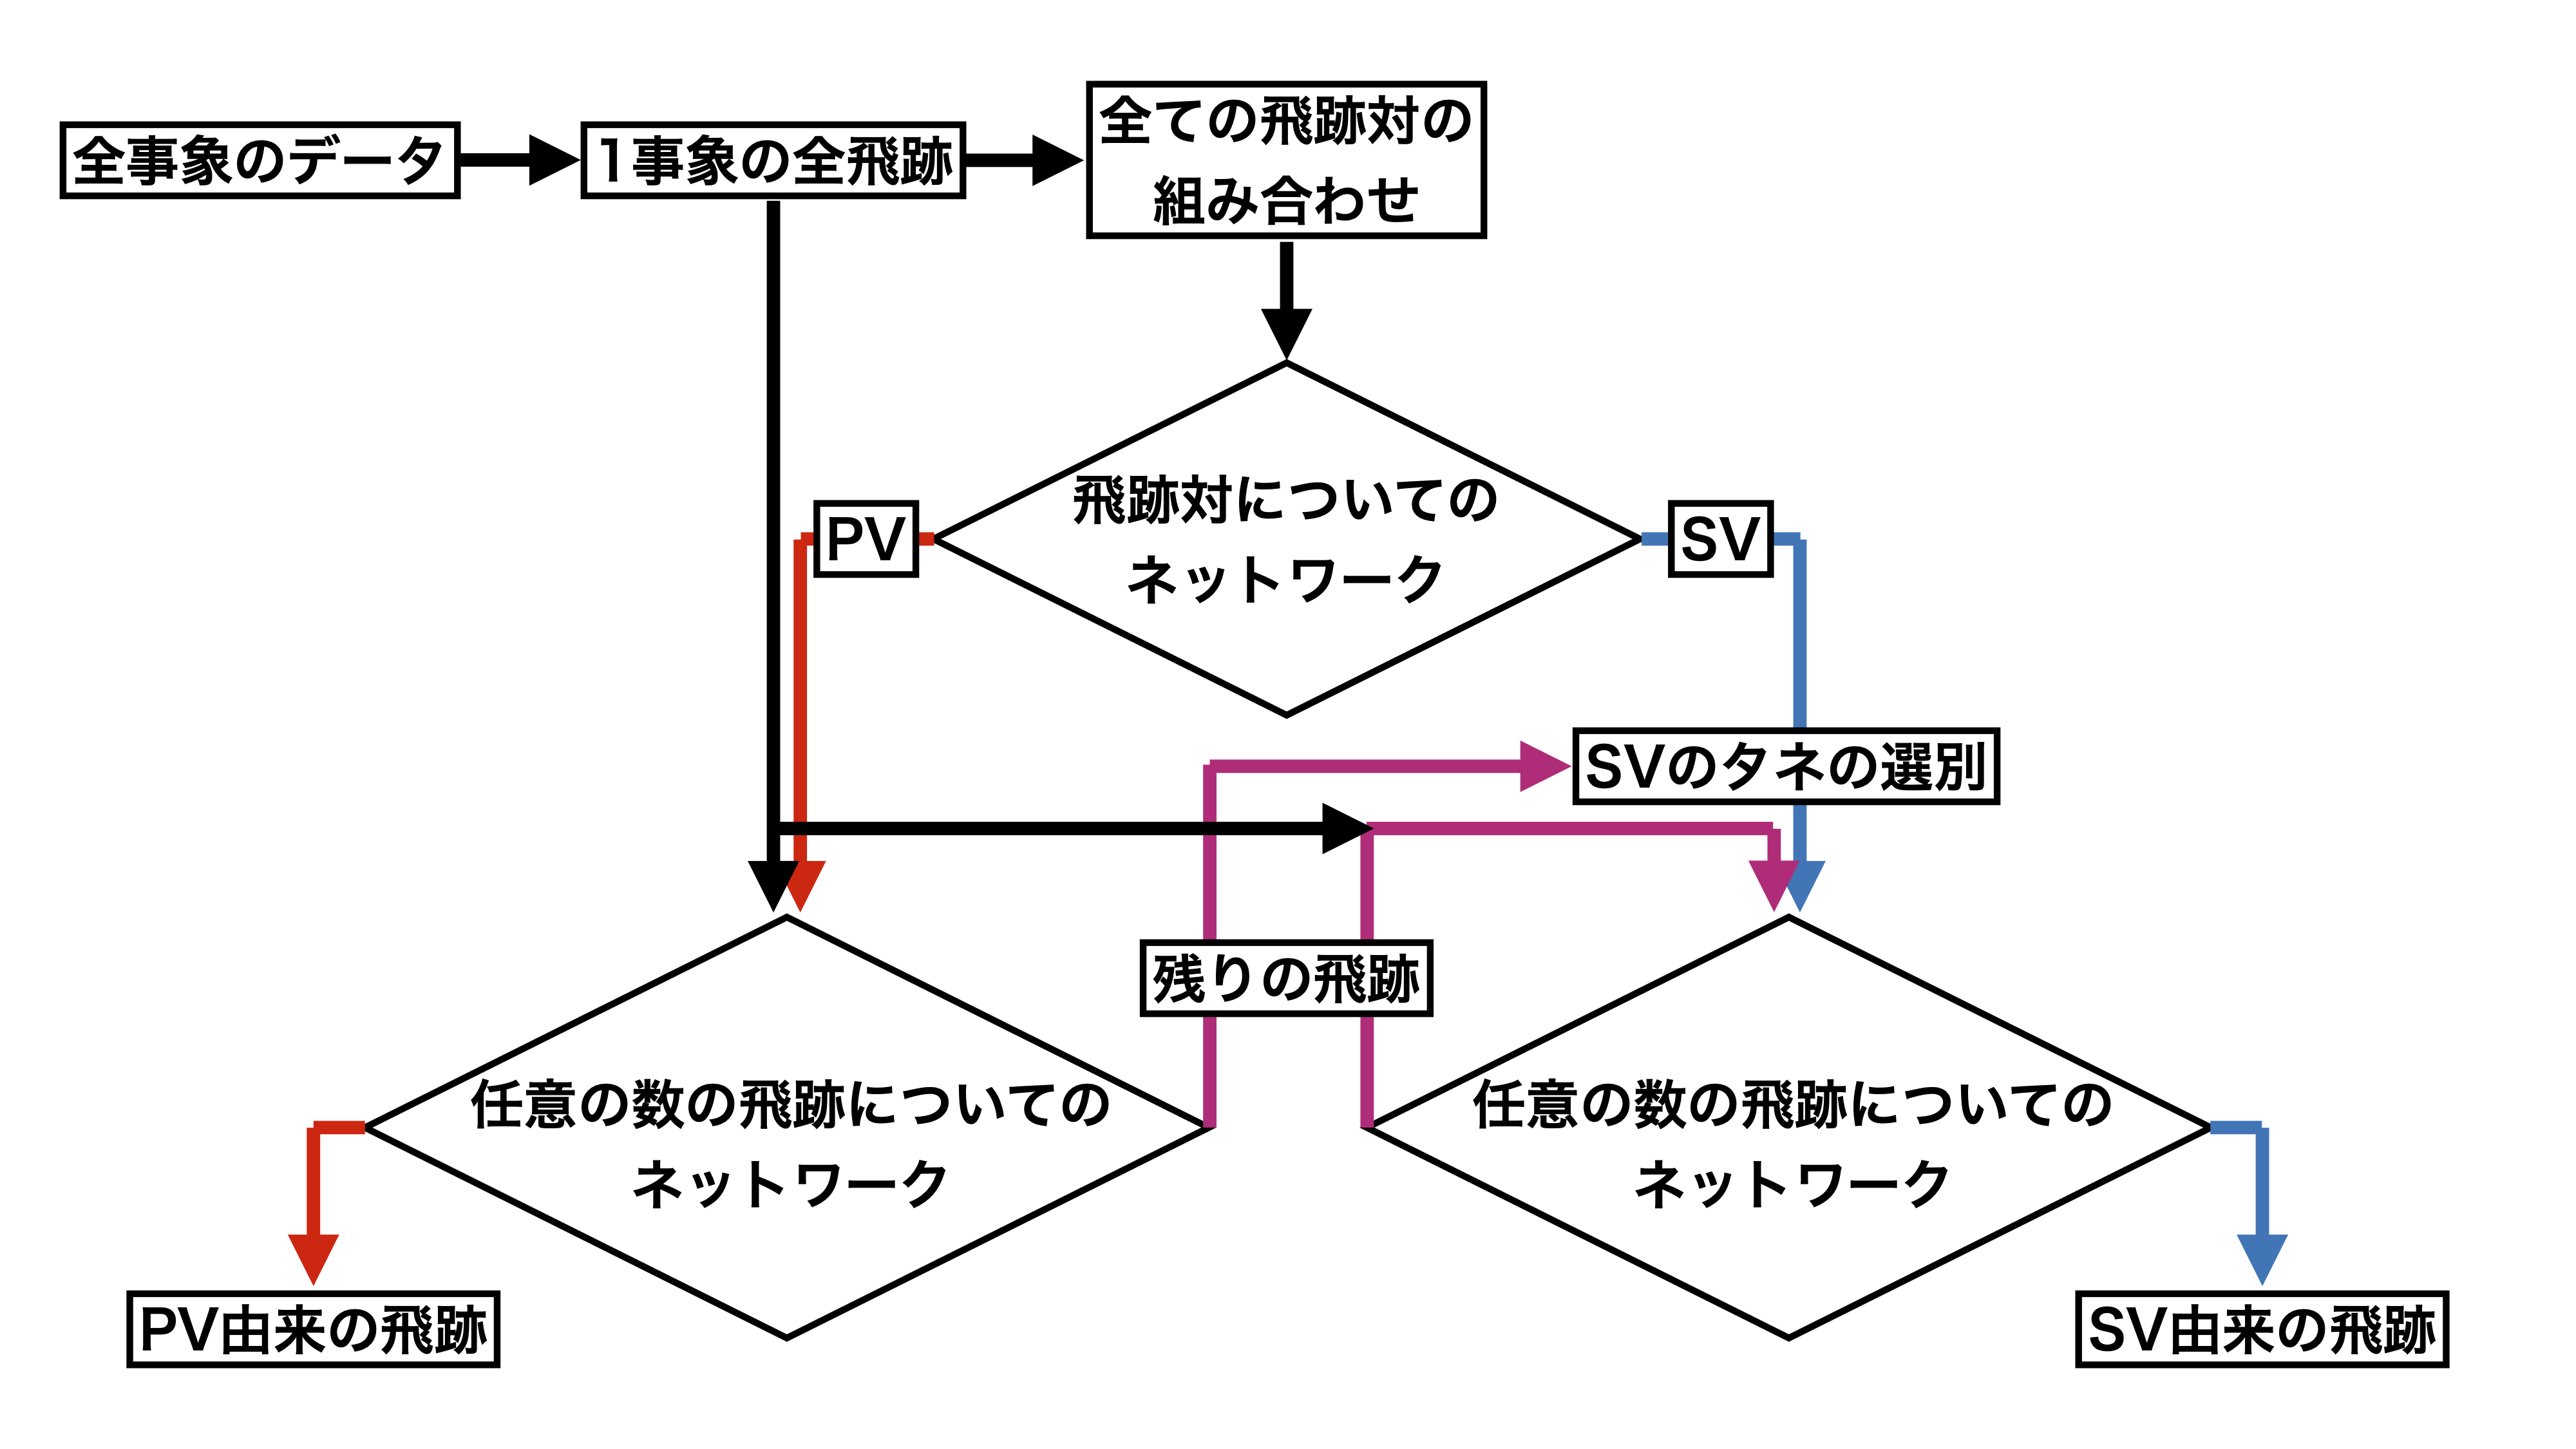
\includegraphics[width=0.9\textwidth, clip]{Figure/4VertexFinderwithDL/4-1-0-1VertexFinderAlgorithm.png}
 \caption{崩壊点検出アルゴリズム}
 \label{4-1-0-1VertexFinderAlgorithm}
\end{figure}

アルゴリズムは以下の手順で崩壊点の再構成を行う。

\begin{enumerate}
 \item 全事象から1事象分のデータを取り出し, 全ての飛跡対の組み合わせを考える。
 \item それら飛跡対に対して, 「飛跡対についてのネットワーク」を使用し, 崩壊点のタネの探索を行う。
 \item SVCC・SVBB・TVCC・SVBCと判定された飛跡対について, 選別を行いsecondary vertexのタネ (SVのタネ) を選ぶ。
 \item PVと判定されたタネ (PVのタネ) について, 「任意の数の飛跡についてのネットワーク」を用いprimary vertexの生成を行う。
 \item SVのタネとprimary vertex由来の飛跡の情報を用い, 「任意の数の飛跡についてのネットワーク」によってSVのタネが無くなるまでSVを生成する。
\end{enumerate}

手順1, 2については飛跡対についてのネットワークの訓練データの作成や学習と全く同様の手順である。

手順3では, 「飛跡対についてのネットワーク」によって得られるSVCC・SVBB・TVCC・SVBCのスコアや崩壊点の位置を用いてより純度の高いSVのタネの集合を作成する。
したがって, SVCC・SVBB・TVCC・SVBCのスコアについての閾値や崩壊点の位置についての最適化が必要である。

手順4では, 「飛跡対についてのネットワーク」によって得られるPVのスコアについて降順に並び替えたPVのタネの集合から個々に「任意の数の飛跡についてのネットワーク」によってprimary vertexを生成する。
ここでは, PVのタネをスコアの高い方から幾つ用いるかについて最適化が必要である。
また一度以上, 「任意の数の飛跡についてのネットワーク」によって結合していると判定された飛跡をprimary vertex由来であると判断している。
この時の「任意の数の飛跡についてのネットワーク」によって得られるスコアについての閾値についてもまた同様に最適化が必要なパラメータである。

手順5について, 手順3で選別したSVのタネと手順4で得られたprimary vertex由来であると判定された飛跡の一覧を用いてsecondary vertexの再構成を行う。
ここでは「任意の数の飛跡についてのネットワーク」のデコーダー部に入力する飛跡から, 再構成されたsecondary vertex由来の飛跡を取り除いて行くことによって, 再帰的にsecondary vertexの生成が行われる。
SVのタネに含まれる飛跡はprimary vertex由来の飛跡の一覧になく, かつそれまでに生成したsecondary vertex由来の飛跡の一覧にもないものを用いる。
このsecondary vertexに関する「任意の数の飛跡についてのネットワーク」のスコアも最適化が必要である。
また, 再構成されたsecondary vertex由来の飛跡の中にprimary vertex由来の飛跡が存在した場合は「任意の数の飛跡についてのネットワーク」によって得られたスコアによって飛跡の争奪が行われる。
手順5はSVのタネが無くなるまで行われ, 再構成されたsecondary vertex由来の飛跡とPV由来の飛跡以外の飛跡は残りの飛跡とする。

以上が崩壊点検出のためのアルゴリズムである。
最適化が必要なパラメータを以下にまとめる。

\begin{itemize}
 \item 「飛跡対についてのネットワーク」によって得られるSVCC・SVBB・TVCC・SVBCのスコアについての閾値
 \item 「飛跡対についてのネットワーク」によって得られる崩壊点の位置についての閾値
 \item 使用するPVのタネの数
 \item primary vertexの生成に関する「任意の数の飛跡についてのネットワーク」によって得られるスコアについての閾値
 \item secondary vertexの生成に関する「任意の数の飛跡についてのネットワーク」によって得られるスコアについての閾値
\end{itemize}


%%%%%%%%%%%%%%%%%%%%%%%%%%%%%%%%%%%%%%%%%%%%%%%%%%%%%%%%%%%%%%%%%%%%%%%%%%%%%%%%%%%%%%%%%%%%%%%%%%%%%
\section{崩壊点検出の最適化と評価} \label{VFDL:TuneandPerformanceofVFDL}

崩壊点検出の最適化では, まず「飛跡対についてのネットワーク」によって得られるSVCC・SVBB・TVCC・SVBCのスコアと崩壊点の位置に関する閾値の最適化を行う。
次に, 使用するPVのタネの数, primary vertex・secondary vertexの生成における「任意の数の飛跡についてのネットワーク」のスコアに関する閾値の最適化を行う。
前者はSVのタネの選別に関するパラメータ, 後者は崩壊点の生成や崩壊点検出の性能についてのパラメータである。


%%%%%%%%%%%%%%%%%%%%%%%%%%%%%%%%%%%%%%%%%%%%%%%%%%%%%%%%%%%%%%%%%%%%%%%%%%%%%%%%%%%%%%%%%%%%%%%%%%%%%
\subsection{SVのタネの選別} \label{VFDL:TPVFDL:SVSeedSelection}

SVのタネを選別する上での評価基準として純度と効率を用いる。
ここでは, SVのタネの効率や純度について, SVCC・SVBB・TVCC・SVBCのスコアの和に対する閾値と崩壊点の位置に関する閾値を変化させ最適な値を探る。
ただし崩壊点検出アルゴリズムでは, ここからprimary vertex由来である飛跡を含むタネを除外する為, その純度は更に改善されると考えられる。
また, SVのタネの選別におけるPre-Selectionとして, 「飛跡対についてのネットワーク」によってNC・PV・Othersと判断された飛跡対を取り除いている。
以上より, SVのタネについての効率と純度を次のように定義する。
\begin{equation}
 \begin{split}
{\rm 効率 = \frac{崩壊点の位置<閾値 \land スコアの和>閾値 \land \overline{NC・PV・Others}}{\overline{NC・PV・Others}}}\\
{\rm 純度 = \frac{崩壊点の位置<閾値 \land スコアの和>閾値 \land \overline{NC・PV・Others}}{崩壊点の位置<閾値 \land スコアの和>閾値}}
 \end{split}
\end{equation}
閾値とSVのタネの効率, 純度の関係を図\ref{4-2-1-1SVSeed}に示す。

\begin{figure}[htbp]
 \centering
 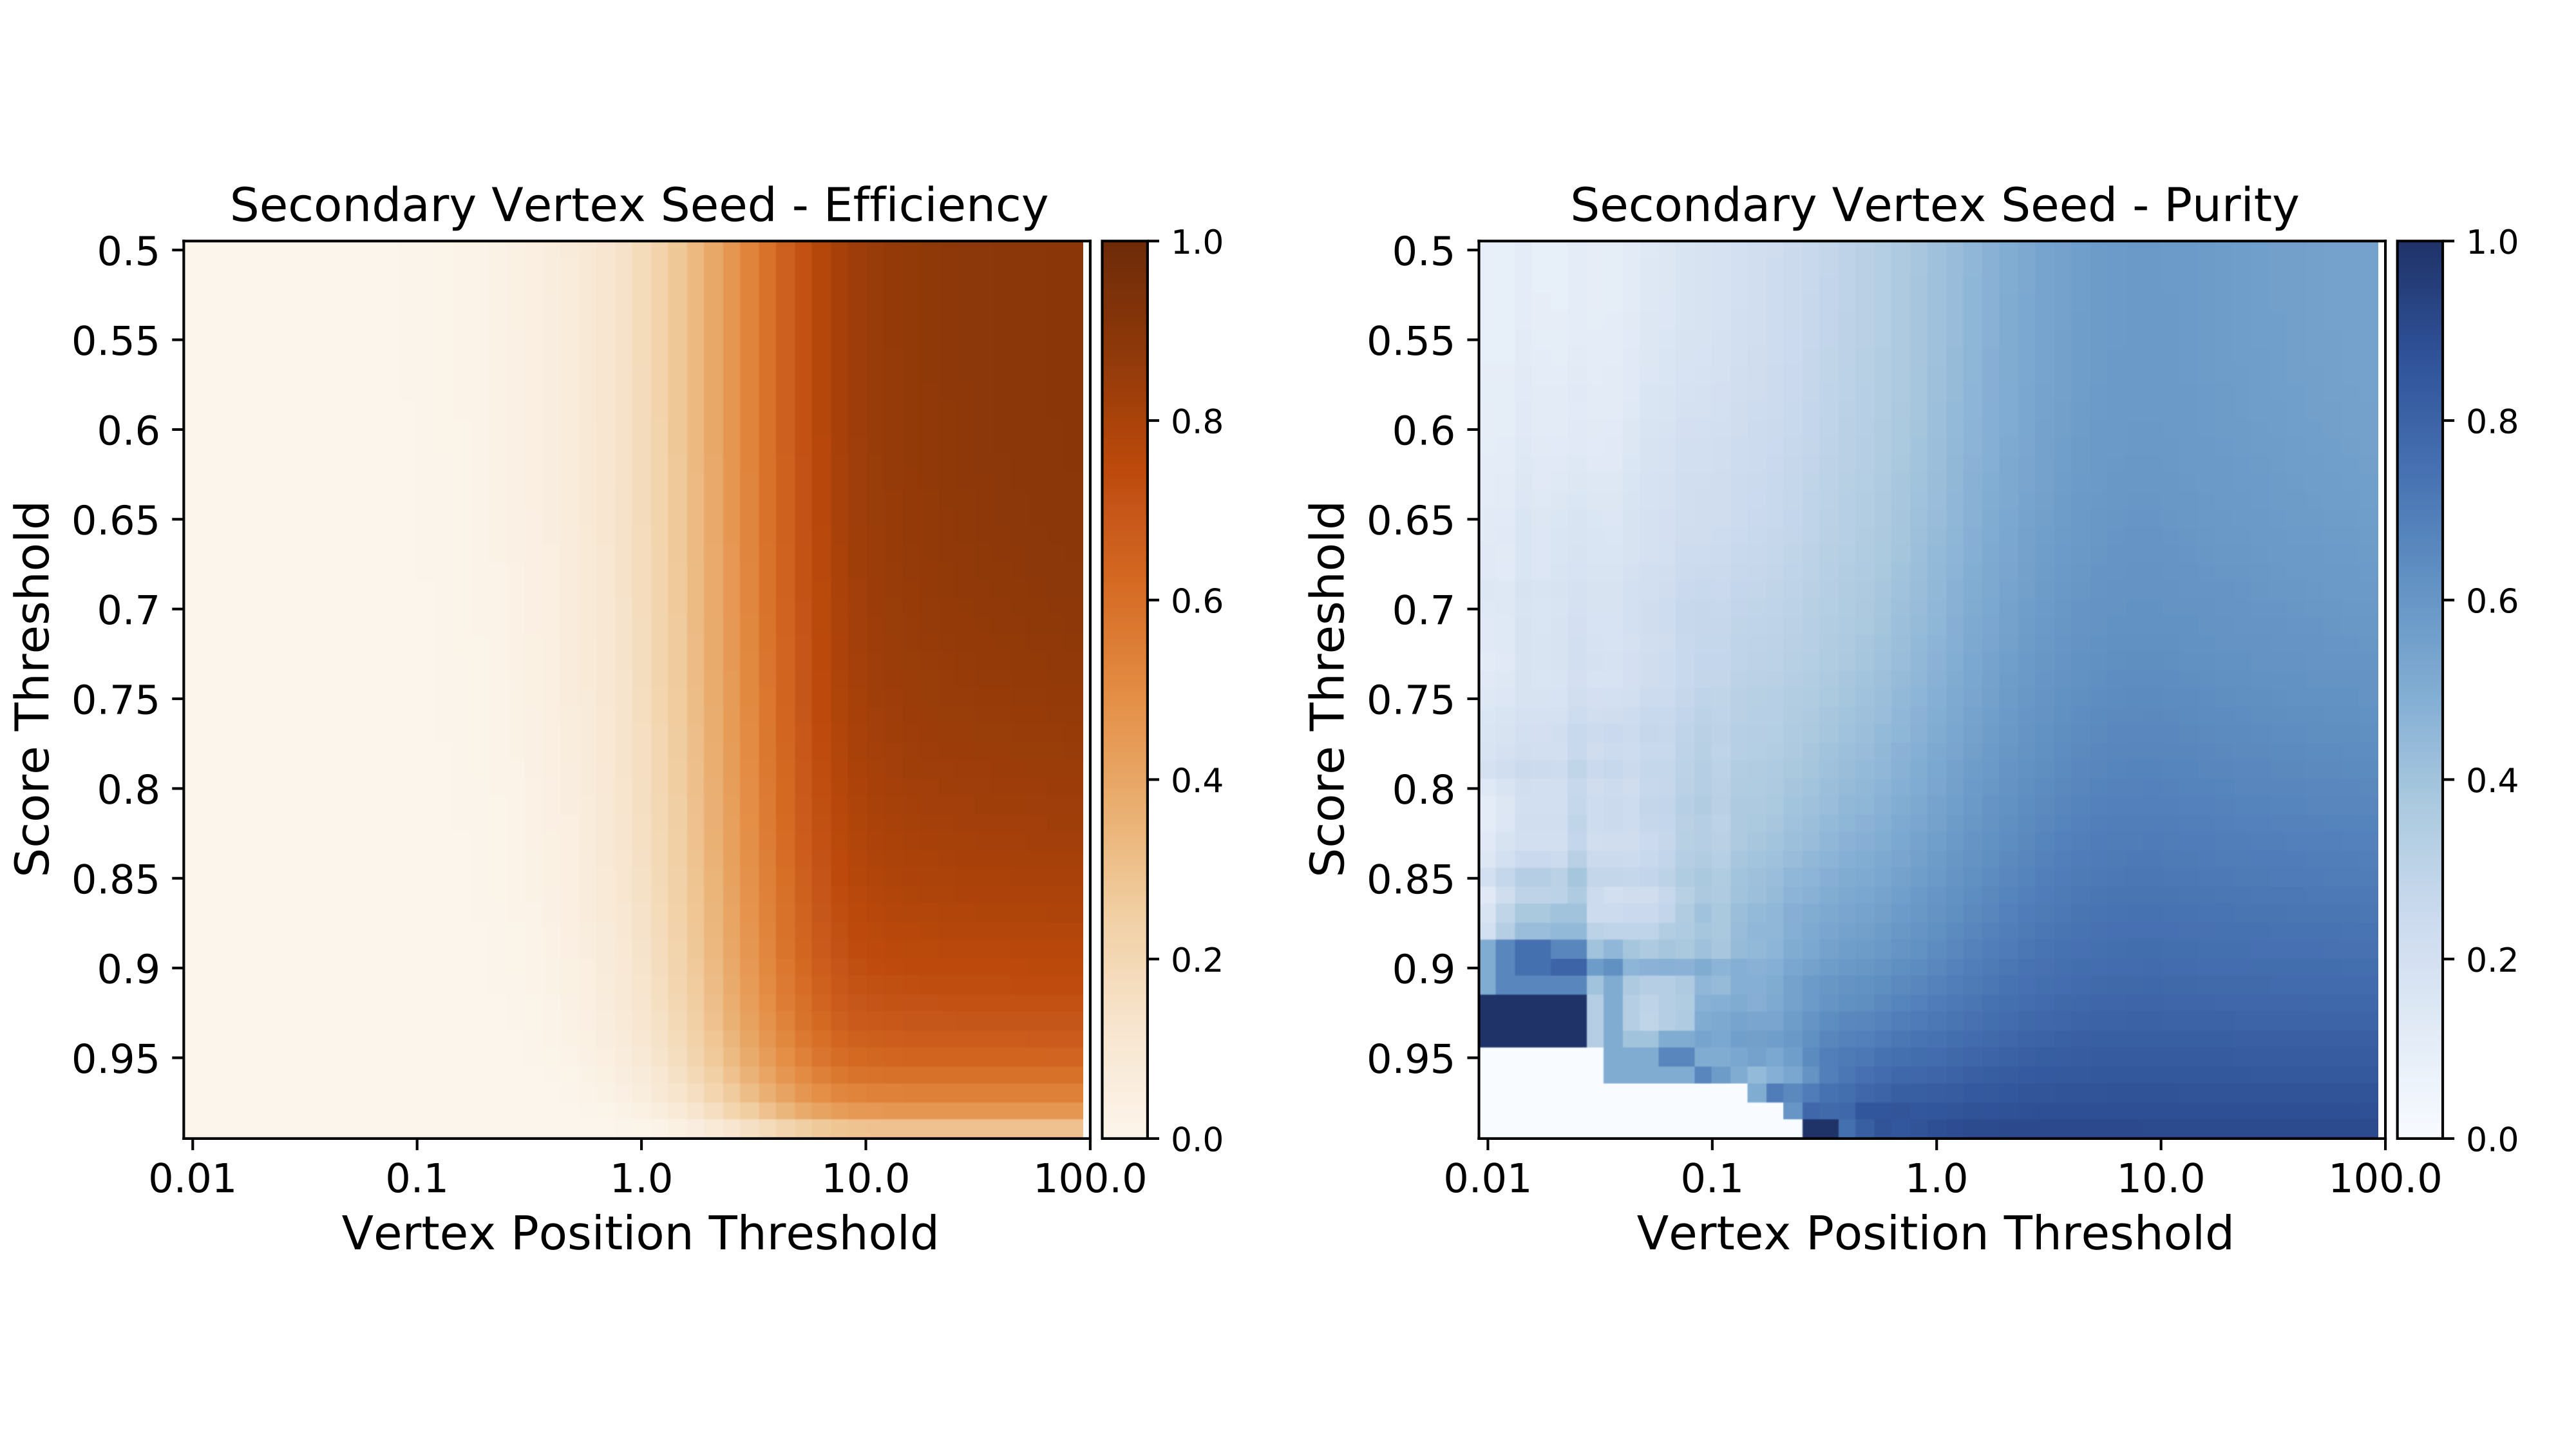
\includegraphics[width=0.9\textwidth, clip]{Figure/4VertexFinderwithDL/4-2-1-1SVSeed.png}
 \caption[閾値とSVのタネの効率, 純度の関係]{閾値とSVのタネの効率, 純度の関係。図左が効率についての関係, 図右が純度についての関係である。縦軸はSVCC・SVBB・TVCC・SVBCのスコアの和に対しての閾値, 横軸は崩壊点の位置についての閾値を示している。また, 横軸についてはログスケールを用いている。}
 \label{4-2-1-1SVSeed}
\end{figure}

効率は崩壊点の位置についての閾値をより大きくすることによって改善されている。
これはsecondary vertexについての崩壊点の位置が$1-10\ \mathrm{mm}$の間でピークを持つことから理解できる。
一方, スコアについての閾値は位置と比較して変化が小さく, $0.8$程度から徐々に効率が減少している。
このことから, SVCC・SVBB・TVCC・SVBCのスコアの和は比較的大きな値を持っていることが理解できる。
純度については, 崩壊点の位置についての閾値が小さく, かつスコアについての閾値が大きな領域においては選択されたSVのタネが存在しなかった為, $0$としている。
また, 全体の傾向として, 崩壊点の位置についての閾値が一定で, スコアについての閾値が大きい領域で純度が高くなっている。
これは, 前述したような崩壊点の位置の特性や深層学習のスコアから明らかな性質である。

最適なパラメータの設定の探索のため, Precision-Recall (PR) 曲線を使用する (図\ref{4-2-1-2PRCurve})。
ここで, Precisionは純度, Recallは効率である。
図\ref{4-2-1-1SVSeed}からも明らかな様に効率は崩壊点の位置についての閾値が$1\ \mathrm{mm}$の辺りで急速に減少している。
したがって, 崩壊点の位置についての閾値が$1\ \mathrm{mm}$以上の場合についてのみ考えることとする。
また, 性能の最大値として効率と純度の和が最大となるパラメータの組み合わせを用いる。
このパラメータは以降の崩壊点の生成や崩壊点検出の性能, 現行の手法との比較に用いる。

\begin{figure}[htbp]
 \centering
 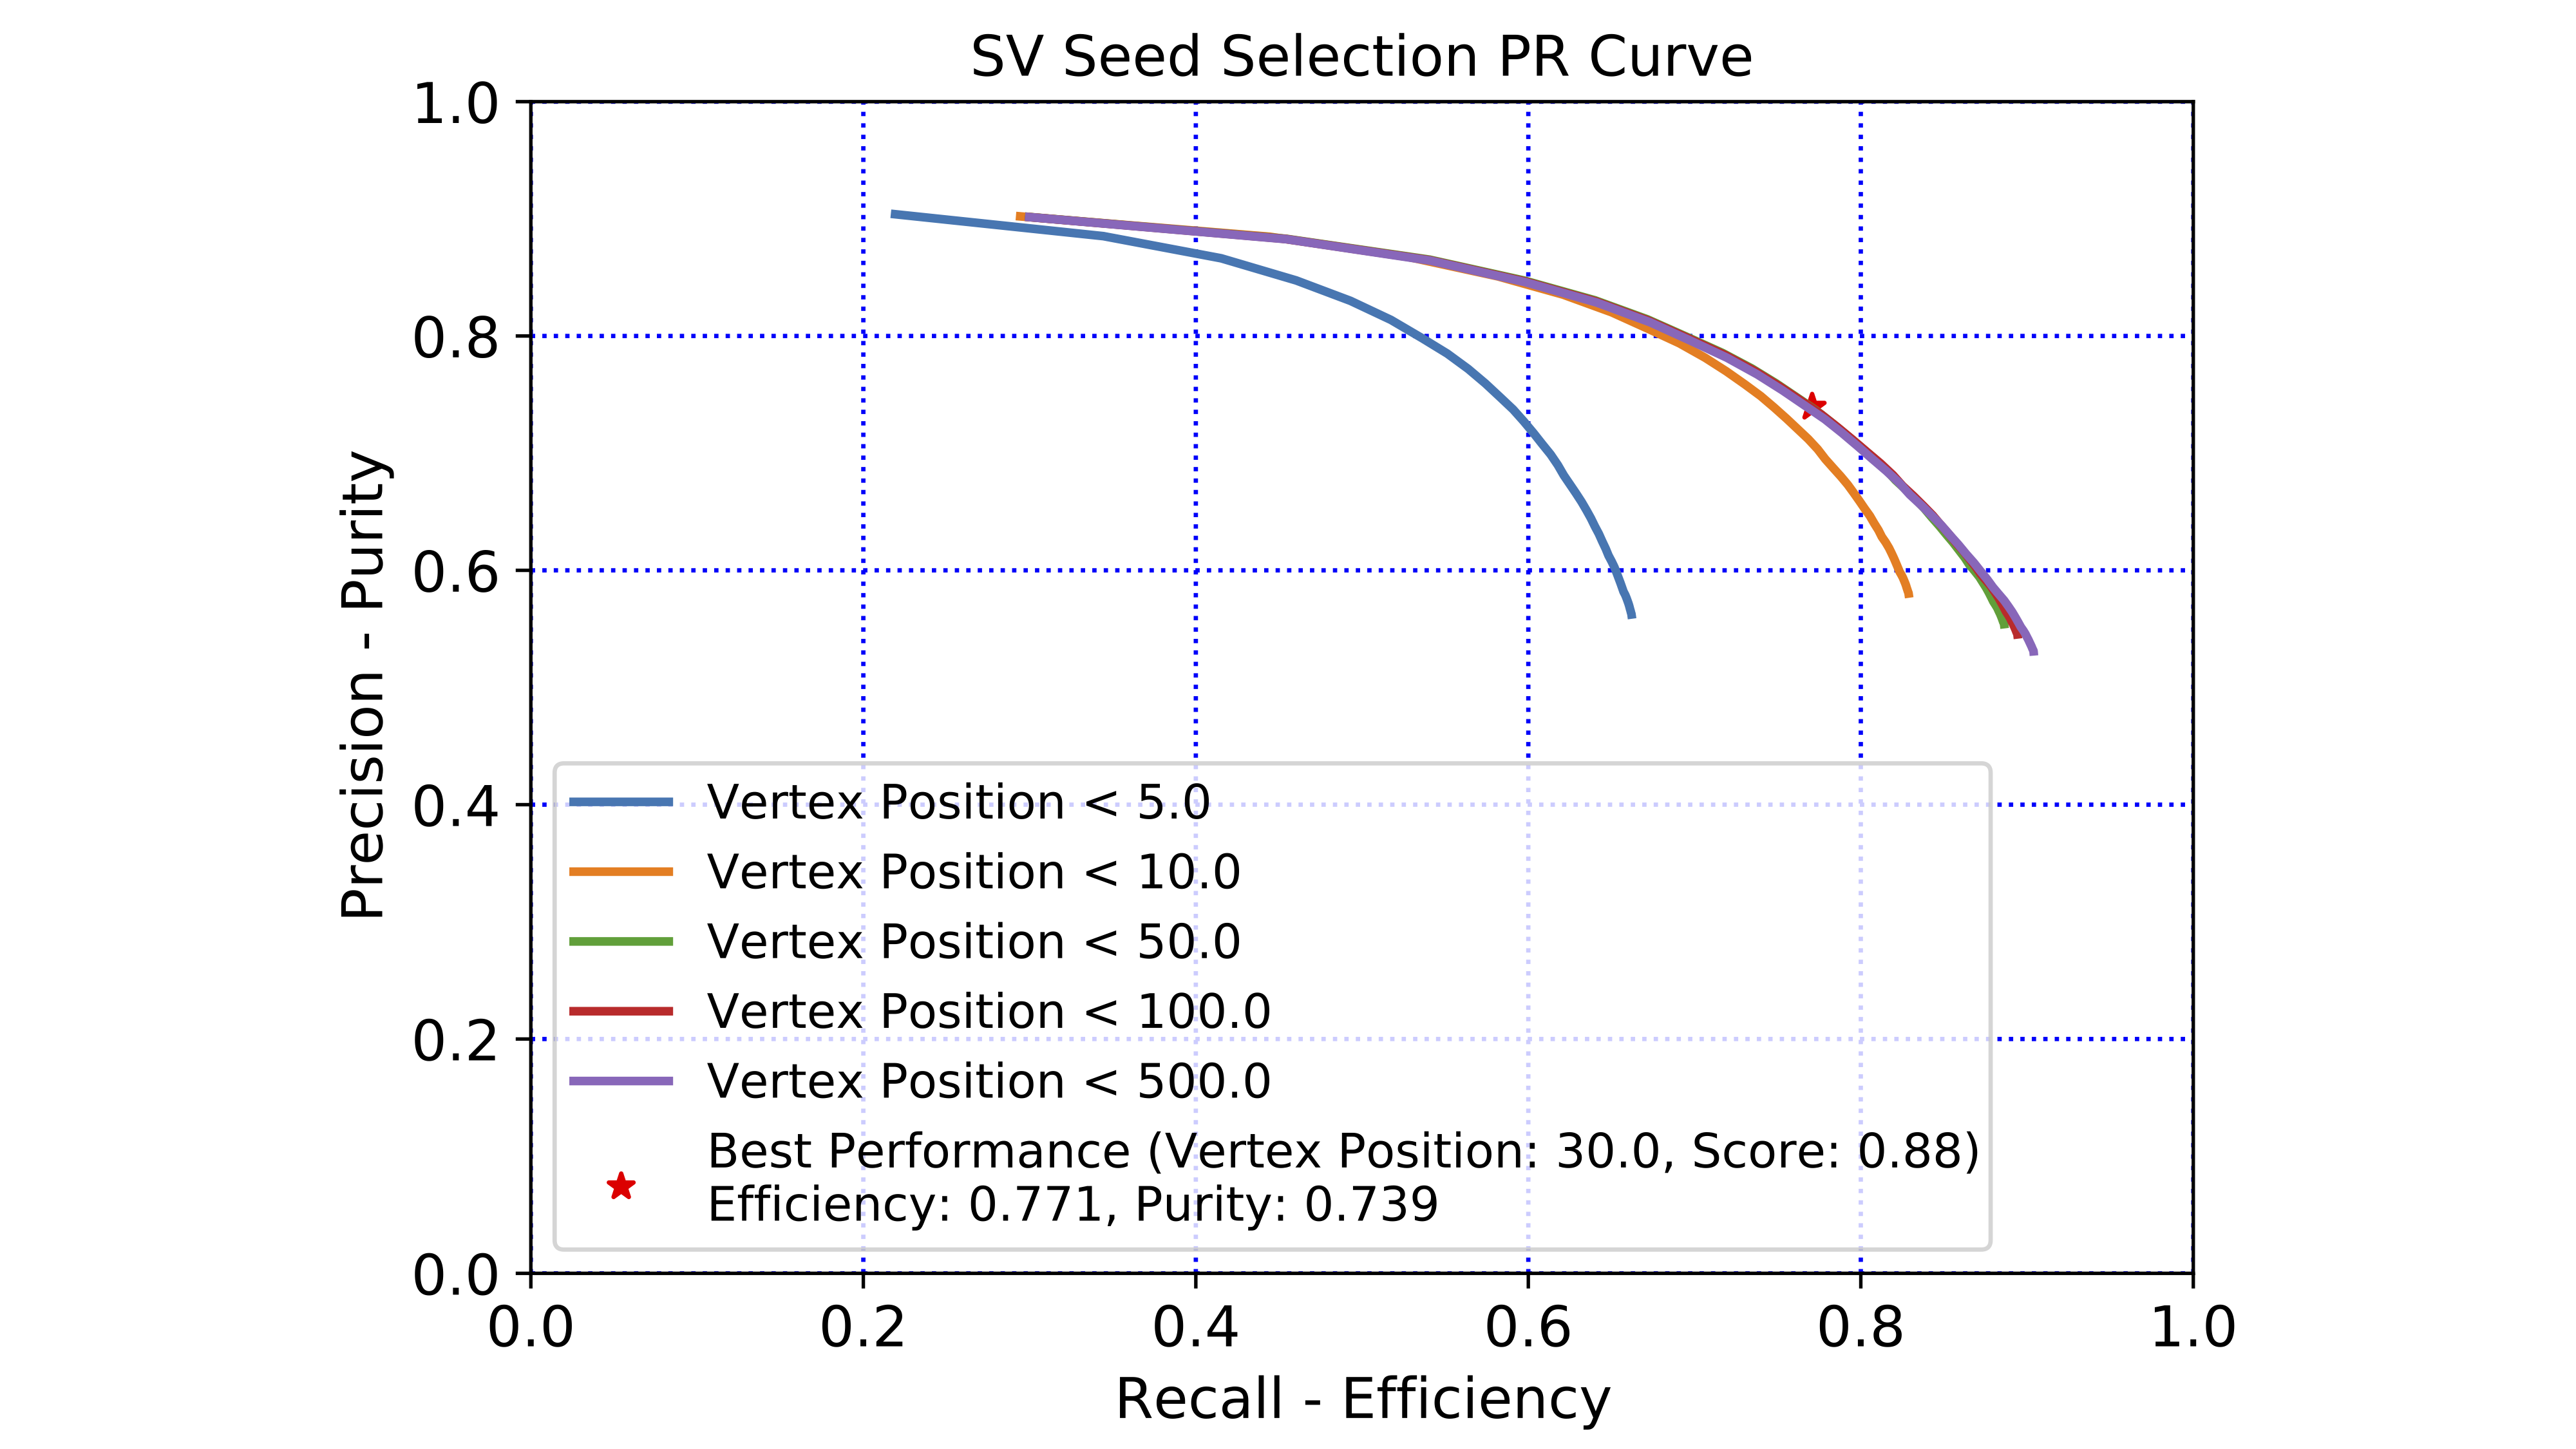
\includegraphics[width=0.9\textwidth, clip]{Figure/4VertexFinderwithDL/4-2-1-2PRCurve.png}
 \caption[閾値とSVのタネの効率, 純度についてのPR曲線]{閾値とSVのタネの効率, 純度についてのPR曲線。縦軸は純度, 横軸は効率である。崩壊点の位置についての閾値を固定し, スコアについての閾値を変化させている。崩壊点の位置については$5.0,\ 10.0,\ 50.0,\ 100.0,\ 500.0\ {\mathrm mm}$のデータのみ描画している。}
 \label{4-2-1-2PRCurve}
\end{figure}

図\ref{4-2-1-2PRCurve}では, 崩壊点の位置については$5.0,\ 10.0,\ 50.0,\ 100.0,\ 500.0\ {\mathrm mm}$のデータのみ描画しているが, 実際には$1.0-9.0$まで$1$刻みずつ, $10.0-90.0$まで$10$刻みずつ$100-900$まで$100$刻みずつのデータについて最適なパラメータの探索を行った。
また, スコアについては$0.50-0.99$まで$0.01$刻みでの探索を行った。
実際には崩壊点の位置についての閾値は$50$程度から殆ど変化はなく, それ以上の離れた位置にSVのタネがほとんど存在していない事がわかる。

%%%%%%%%%%%%%%%%%%%%%%%%%%%%%%%%%%%%%%%%%%%%%%%%%%%%%%%%%%%%%%%%%%%%%%%%%%%%%%%%%%%%%%%%%%%%%%%%%%%%%
\subsection{崩壊点の生成} \label{VFDL:TPVFDL:VertexProduction}

崩壊点の生成や崩壊点検出の性能についてのパラメータを最適化する為, その性能を定める評価項目を定義する必要がある。
そのような評価項目としてsecondary vertexの再構成についての効率を用いる。
まず以下の様な評価項目を設ける。

\begin{itemize}
 \item Primary : MC情報によってprimary vertex由来であるとラベルされた飛跡
 \item Bottom : MC情報によってボトム・フレーバーのsecondary vertex由来であるとラベルされた飛跡
 \item Charm : MC情報によってチャーム・フレーバーのsecondary vertex由来であるとラベルされた飛跡
  \item Others : MC情報によってOthersであるとラベルされた飛跡
\end{itemize}

これらについてどの程度ネットワークがsecondary vertexと判断してしまったかを評価する。
PrimaryやOthersはsecondary vertexではない為, 値が小さいほど性能が高くsecondary vertexの純度が高いと判断する。
BottomやCharmはsecondary vertexである為, 値が大きいほど性能が高くsecondary vertexの効率が高いと判断する。
更に, BottomやCharmに関しては以下の様な複数個のsecondary vertexを跨いで飛跡を獲得した場合の罰則を考慮する。

\begin{itemize}
 \item 同一の崩壊チェイン : 同一の崩壊チェイン由来の飛跡のみで構成されているか
 \item 同一の親粒子 : 同一の親粒子由来の飛跡のみで構成されているか
\end{itemize}

ここでは, ボトム・フレーバー, チャーム・フレーバーのsecondary vertexの内, 同じボトム・ハドロンから生じたsecondary vertexの組みを崩壊チェインと呼び, 更に細かく個々のフレーバーのハドロンを親粒子と呼んでいる (図\ref{4-2-2-1SameChainSameParticle})。
同一の崩壊チェイン, 同一の親粒子とはこれらの崩壊チェインや親粒子を跨いで飛跡を選択しているかどうかを判断している。

\begin{figure}[htbp]
 \centering
 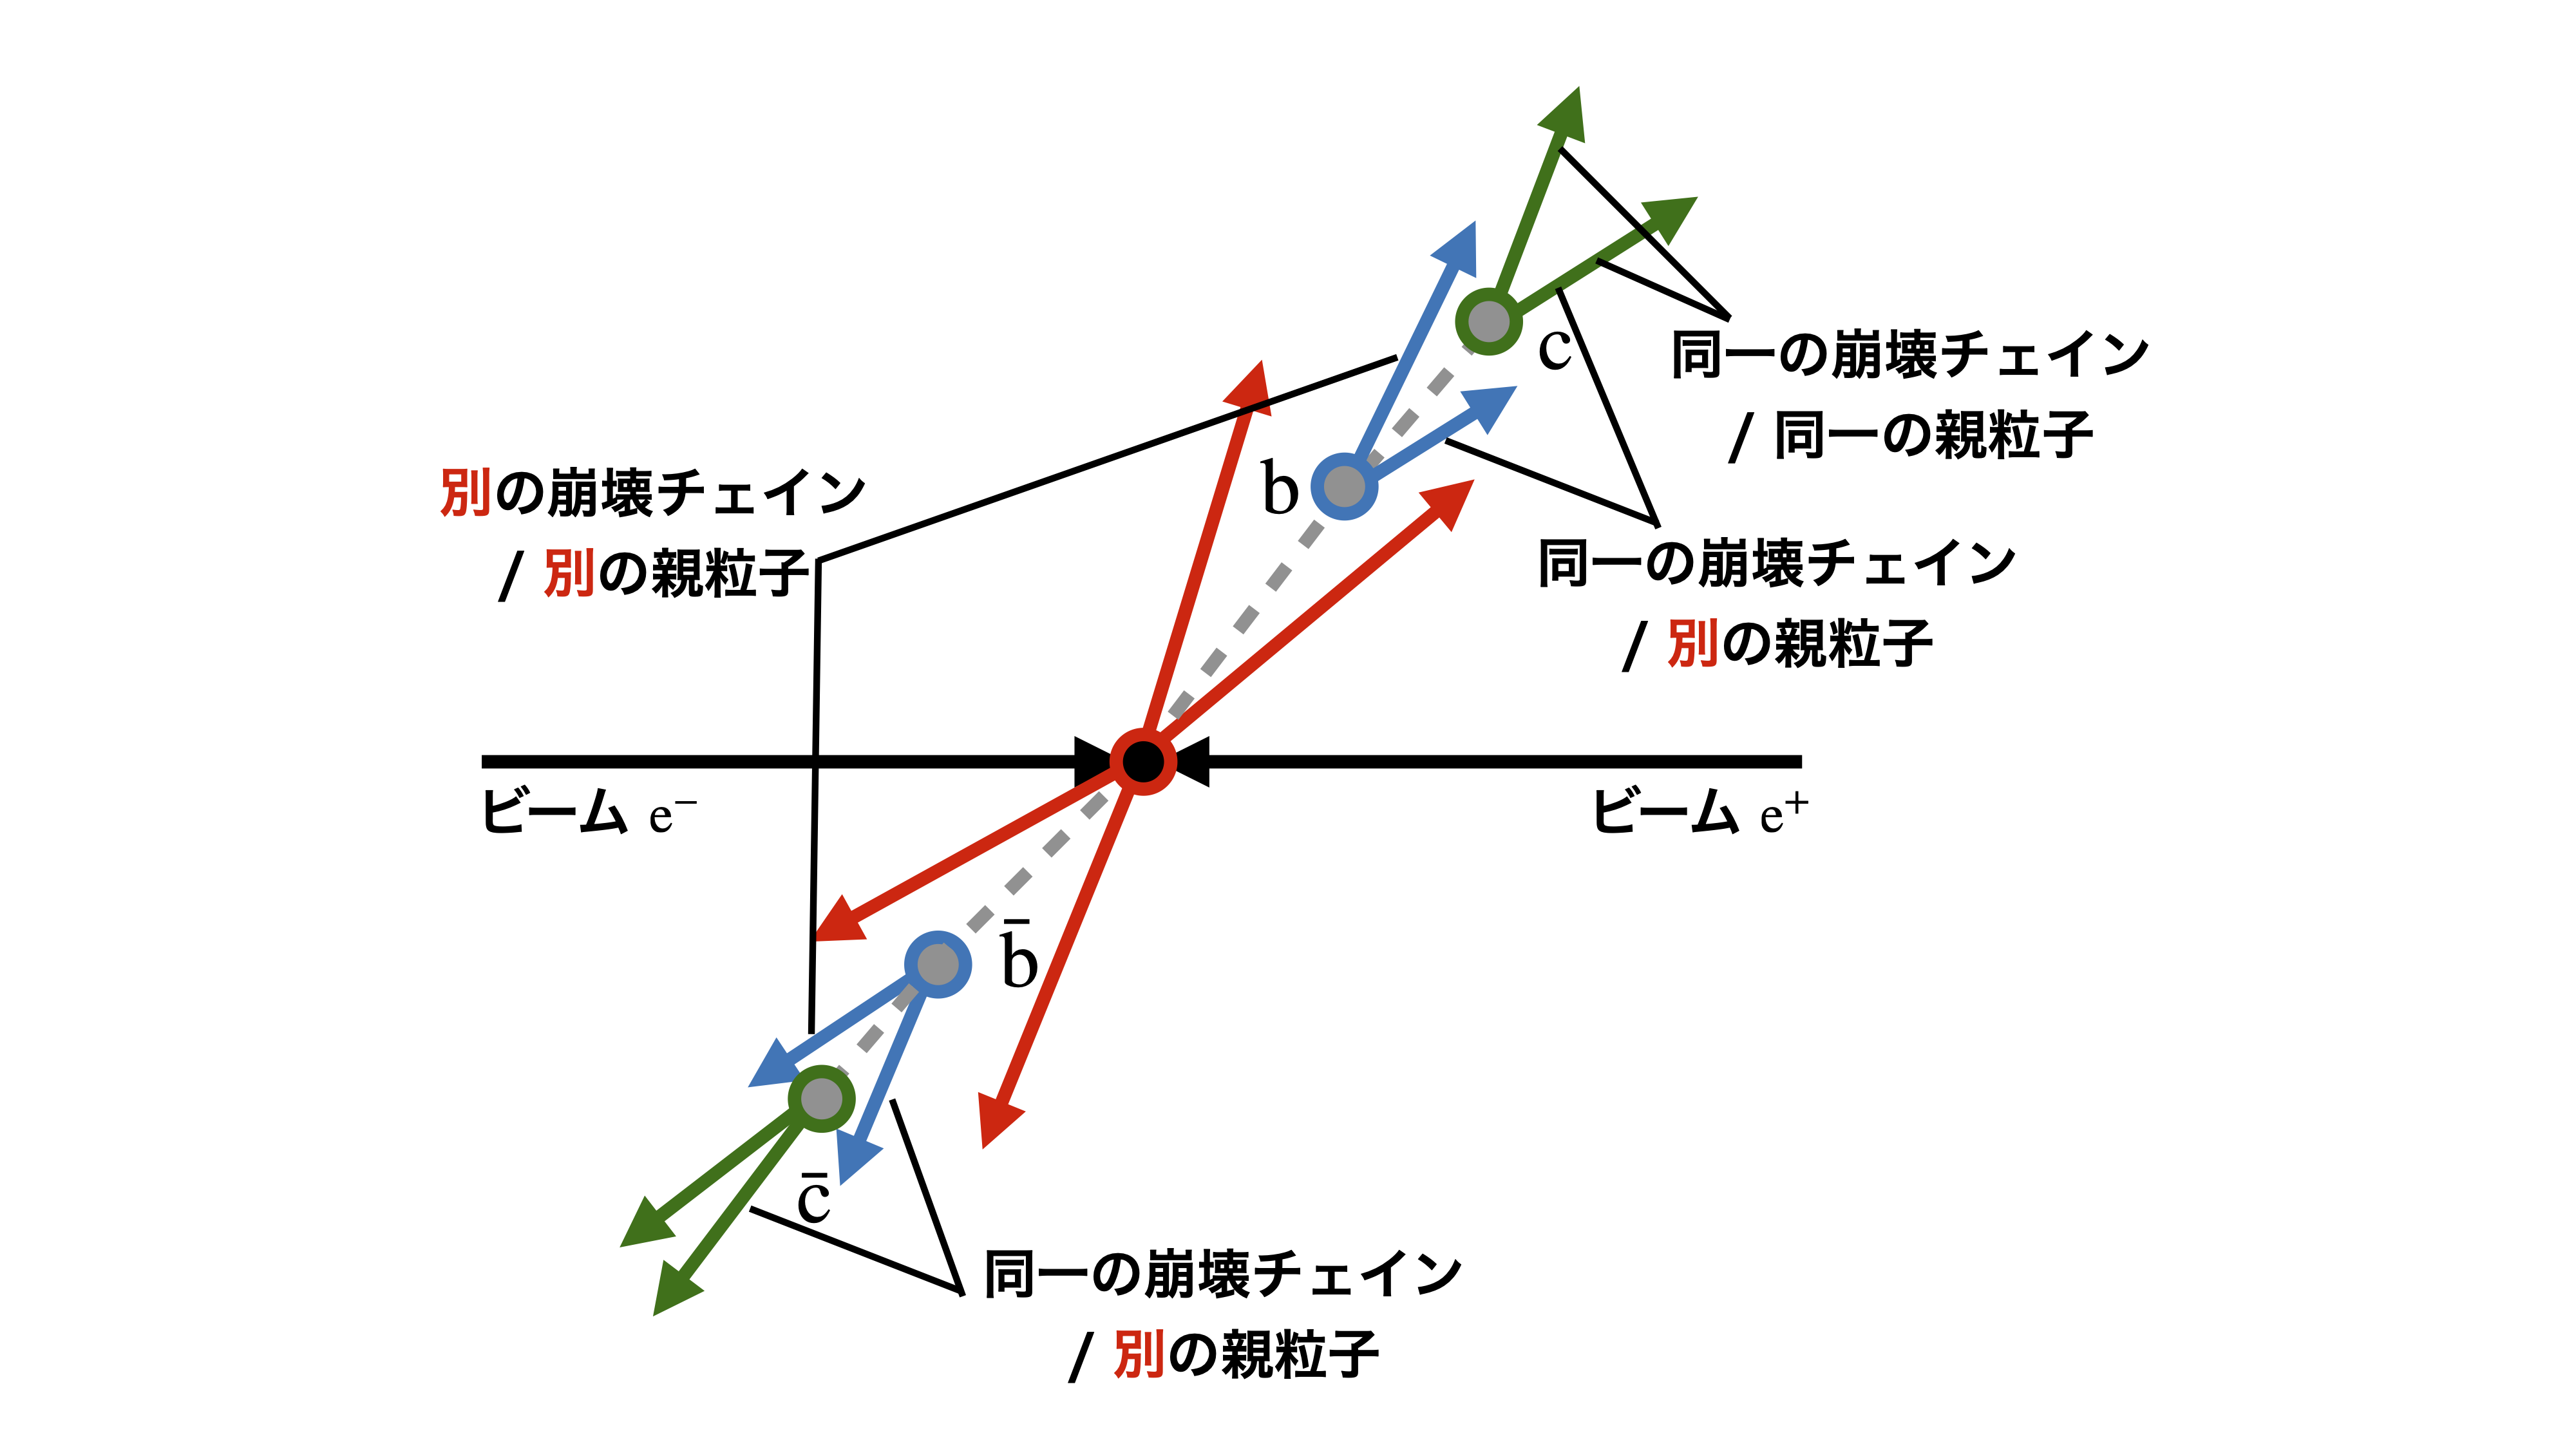
\includegraphics[width=0.9\textwidth, clip]{Figure/4VertexFinderwithDL/4-2-2-1SameChainSameParticle.png}
 \caption[同一の崩壊チェインと同一の親粒子]{同一の崩壊チェインと同一の親粒子}
 \label{4-2-2-1SameChainSameParticle}
\end{figure}

これらの評価項目は前述した現行の手法であるLCFIPlusでの評価項目と同じものである。

崩壊点の生成についてのパラメータは使用するPVのタネの数, primary vertex・secondary vertexの生成におけるネットワークのスコアの閾値の三つである。
それぞれ三つのパラメータについて, PVのタネの数を$1$から$3$個まで, primary vertex・secondary vertexのスコアの閾値を$0.50$から$0.95$まで$0.05$ずつ変化させ, 各評価項目の値を確認する。
データは$100$事象分の飛跡を用いた。
PVのタネを一つ使用した場合の結果を図\ref{4-2-2-2TrackEfficiency}に示す。

\begin{figure}[htbp]
 \centering
  %\begin{tabular}{cccc}
  \begin{minipage}{0.95\textwidth}
   \centering
    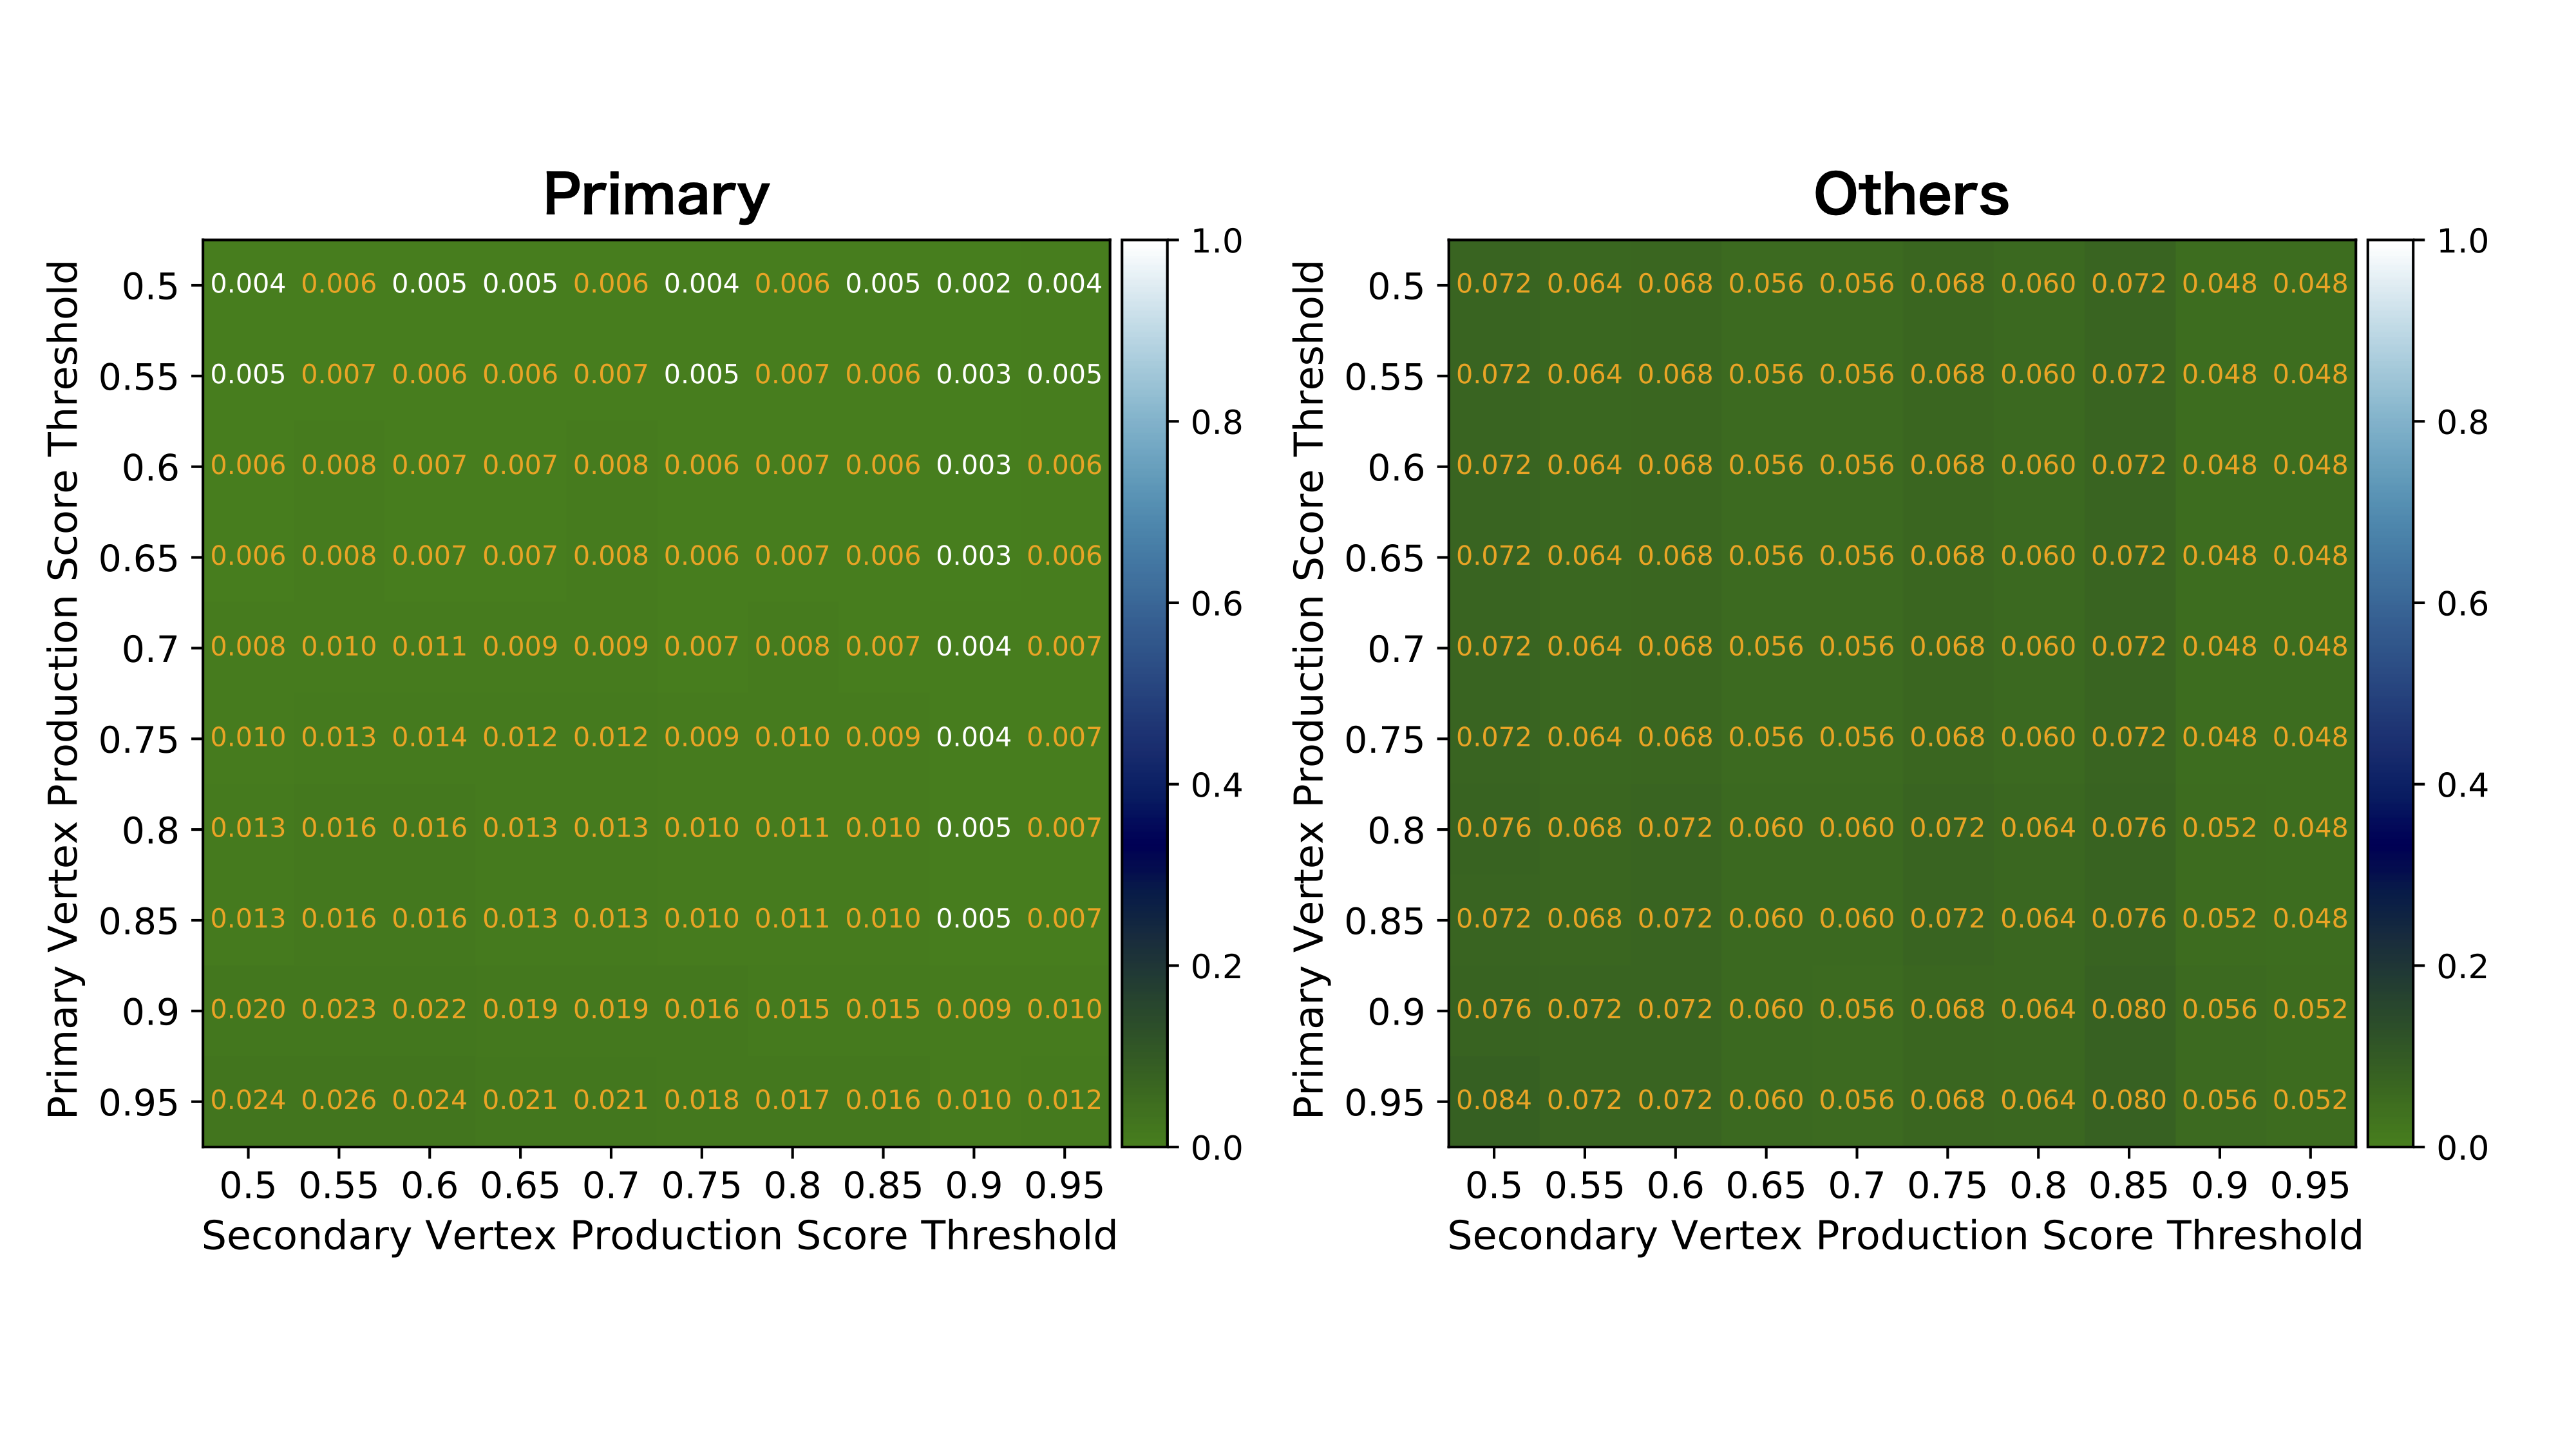
\includegraphics[trim = 0 140 0 125, width=0.9\textwidth, clip]{Figure/4VertexFinderwithDL/4-2-2-2PrimaryOthers.png}
   \end{minipage}
   
   \begin{minipage}{0.95\textwidth}
   \centering
    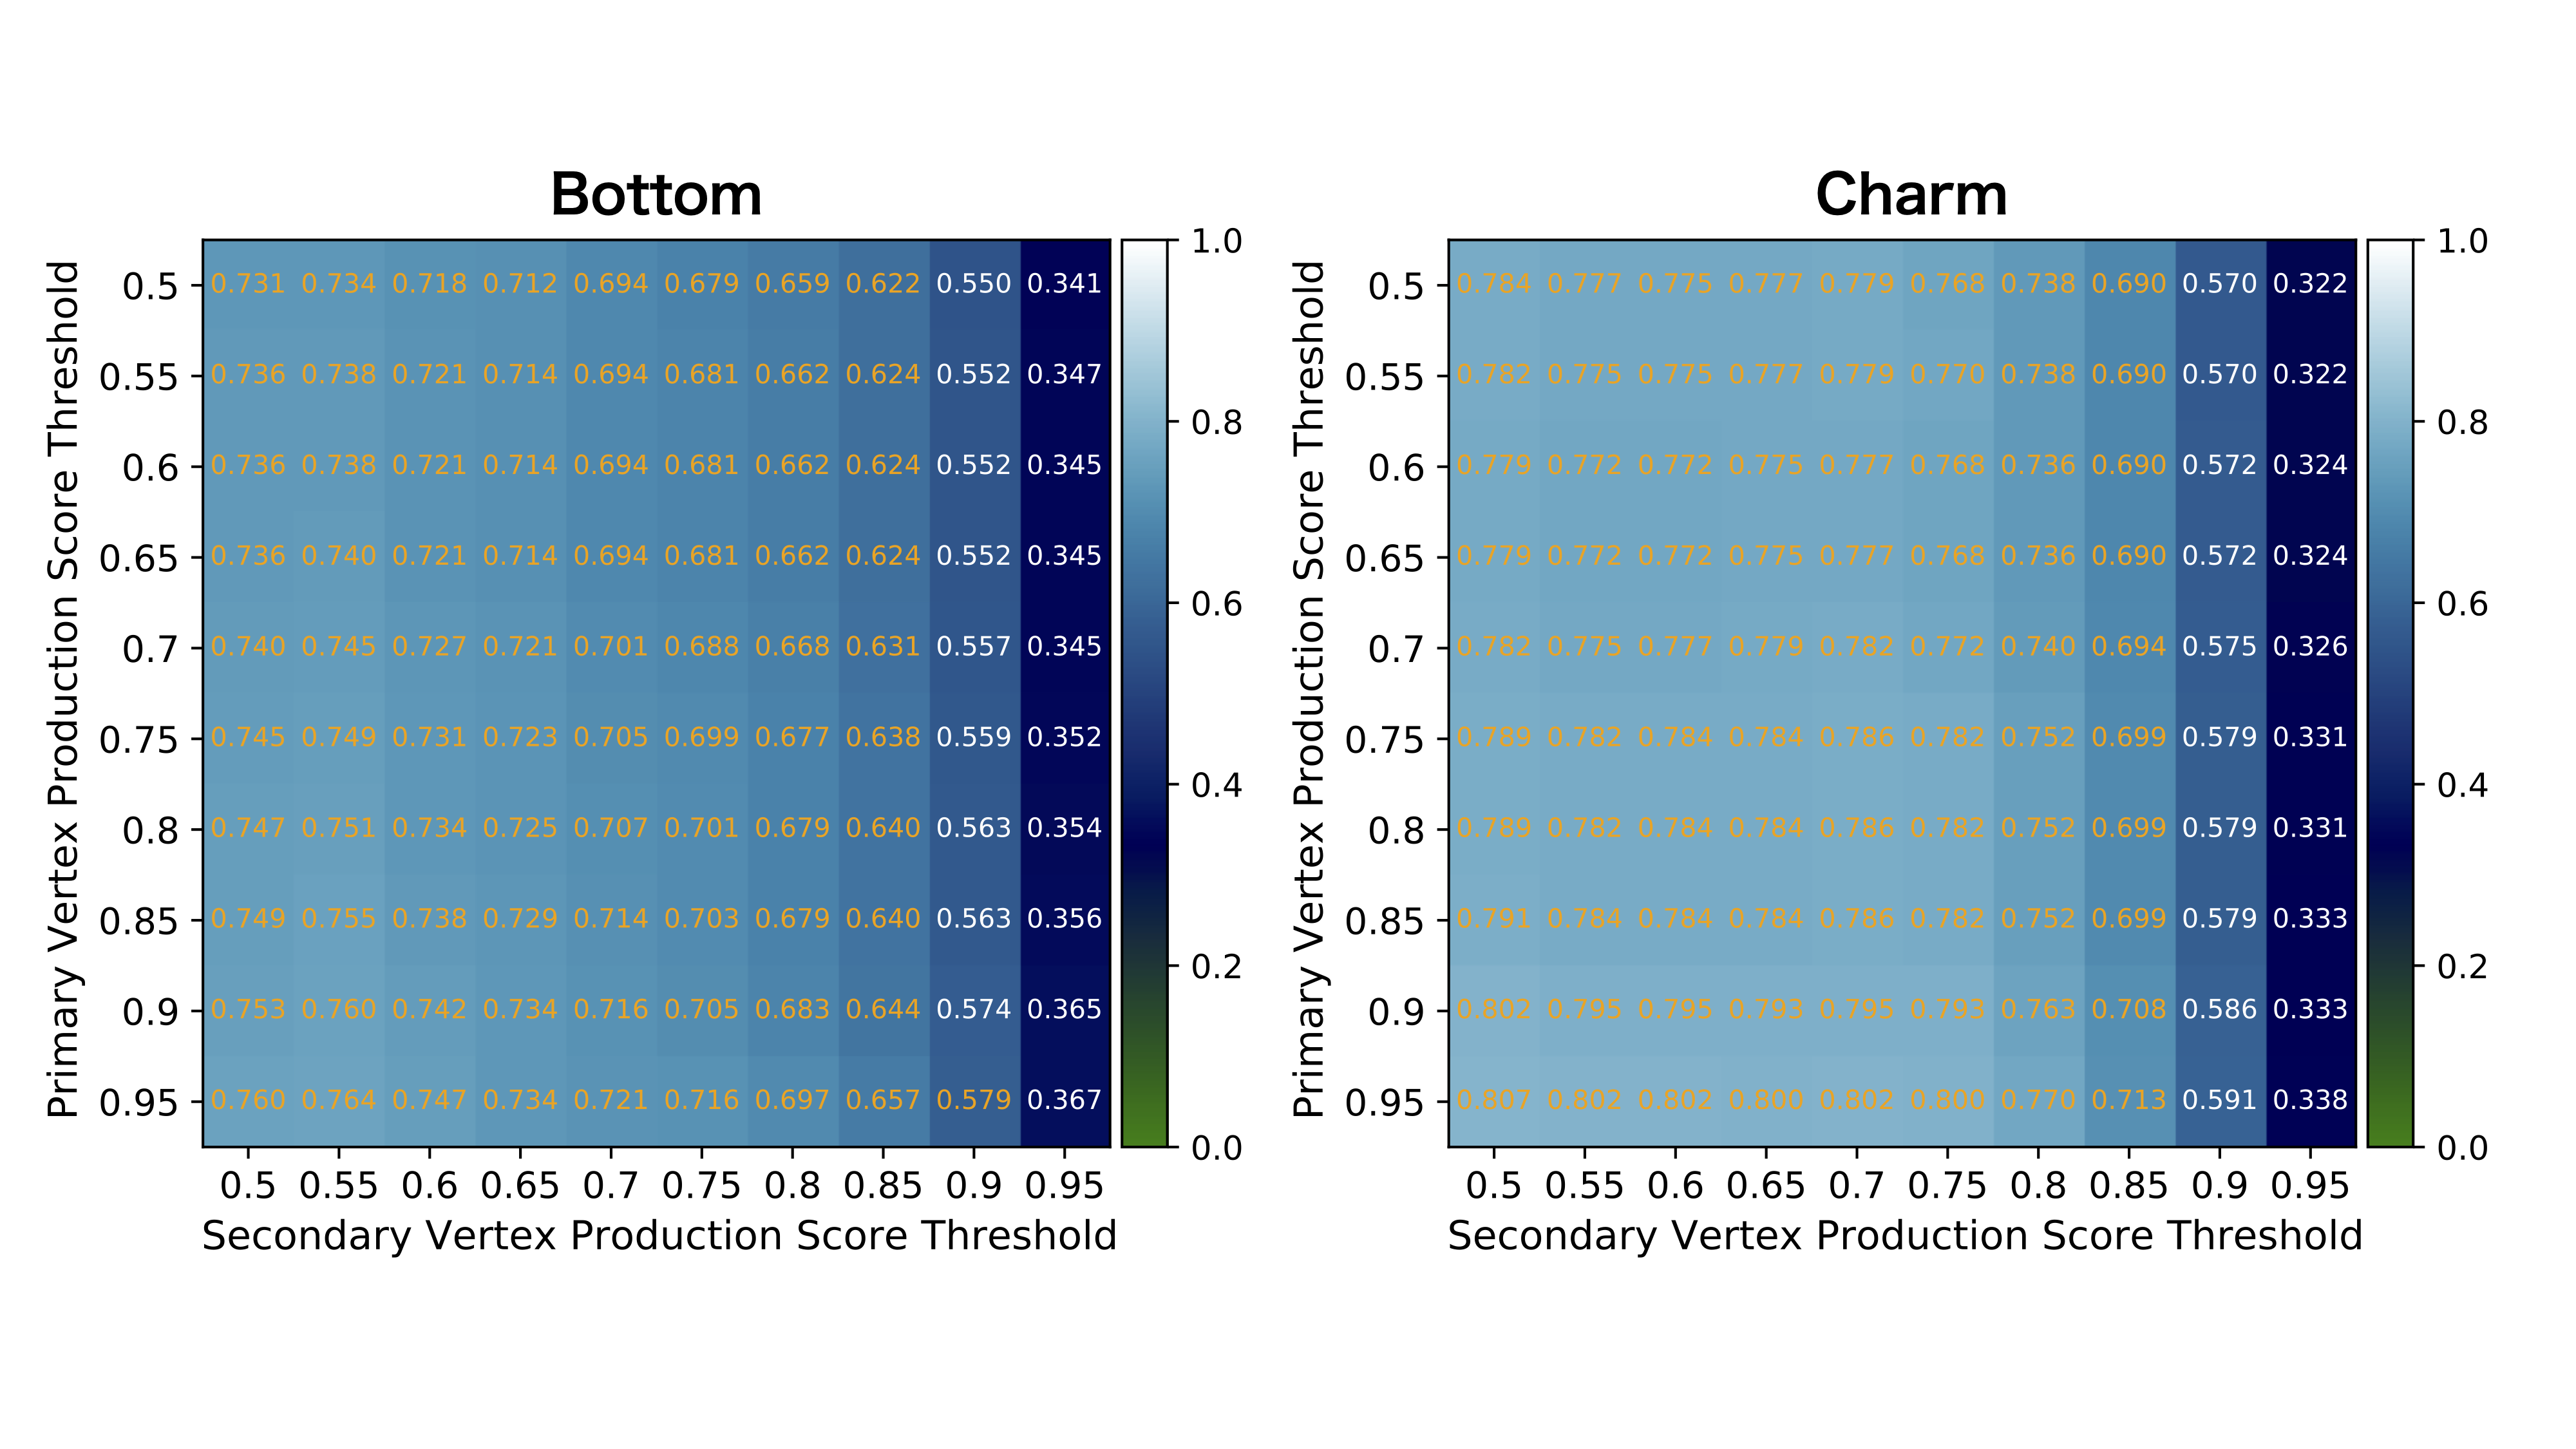
\includegraphics[trim = 0 140 0 125, width=0.9\textwidth, clip]{Figure/4VertexFinderwithDL/4-2-2-2BottomCharm.png}
   \end{minipage}
   
   \begin{minipage}{0.95\textwidth}
   \centering
    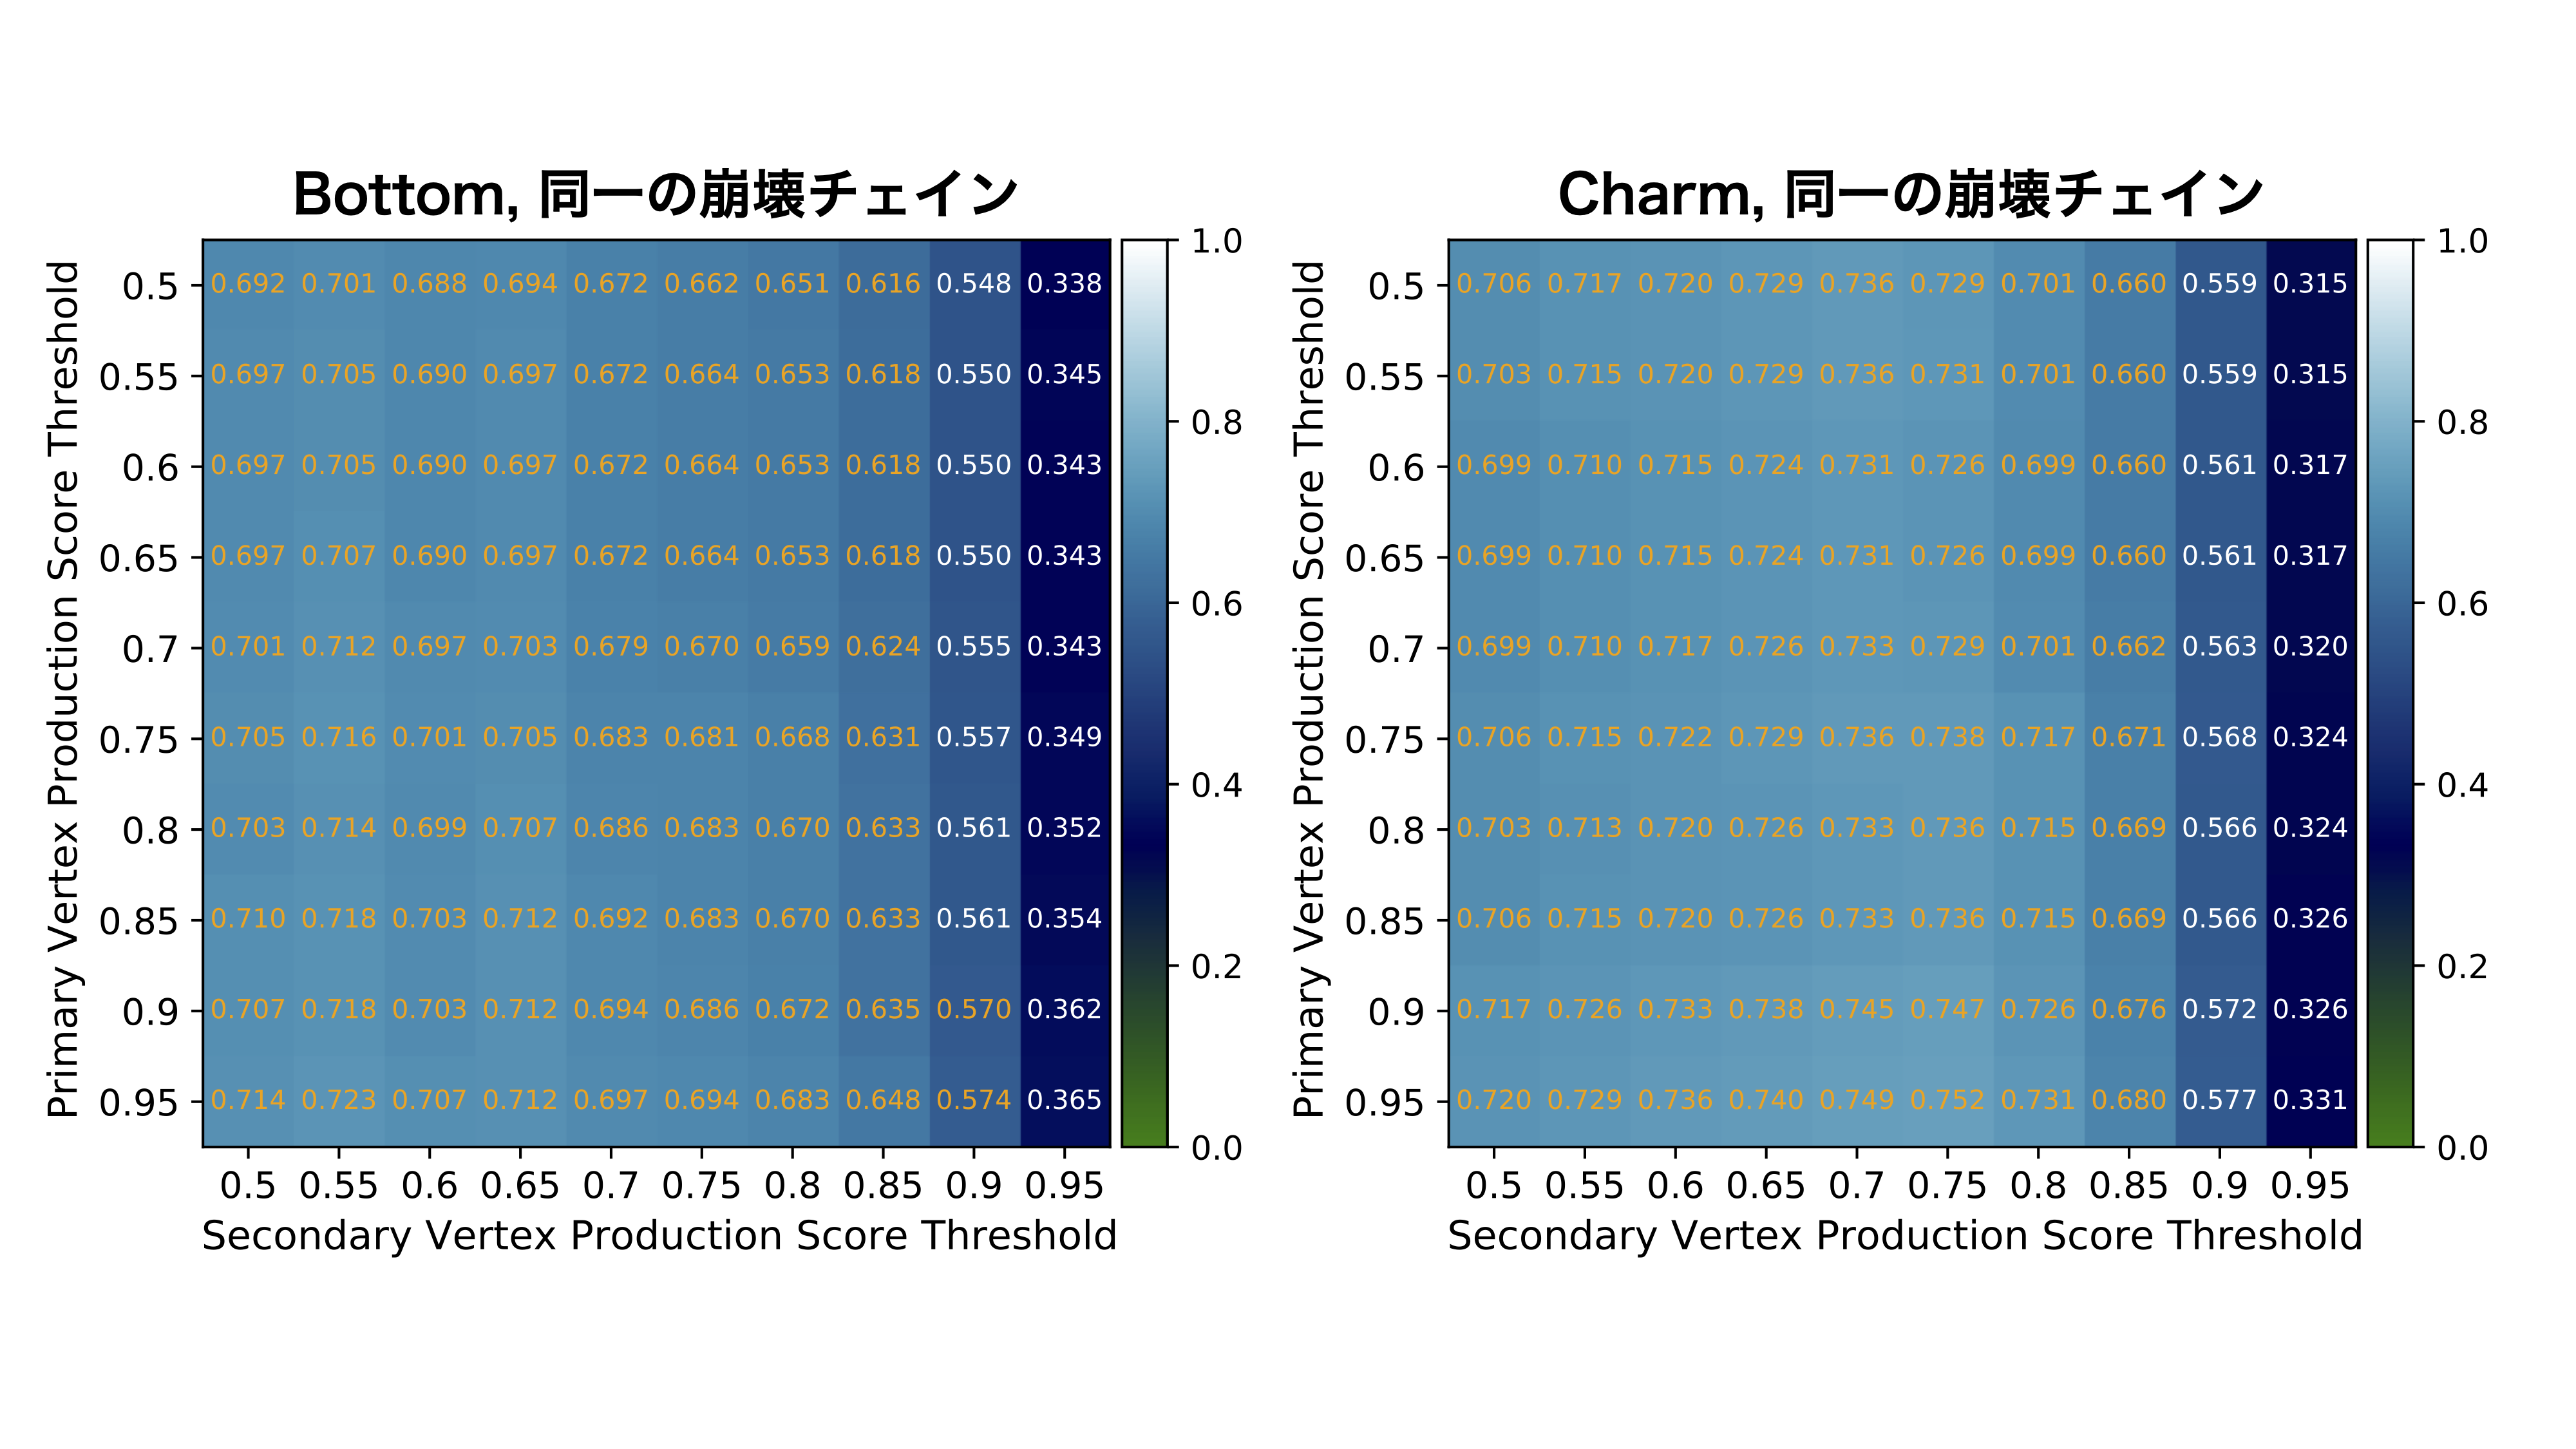
\includegraphics[trim = 0 140 0 125, width=0.9\textwidth, clip]{Figure/4VertexFinderwithDL/4-2-2-2SameDecayChain.png}
   \end{minipage}
   
   \begin{minipage}{0.95\textwidth}
   \centering
    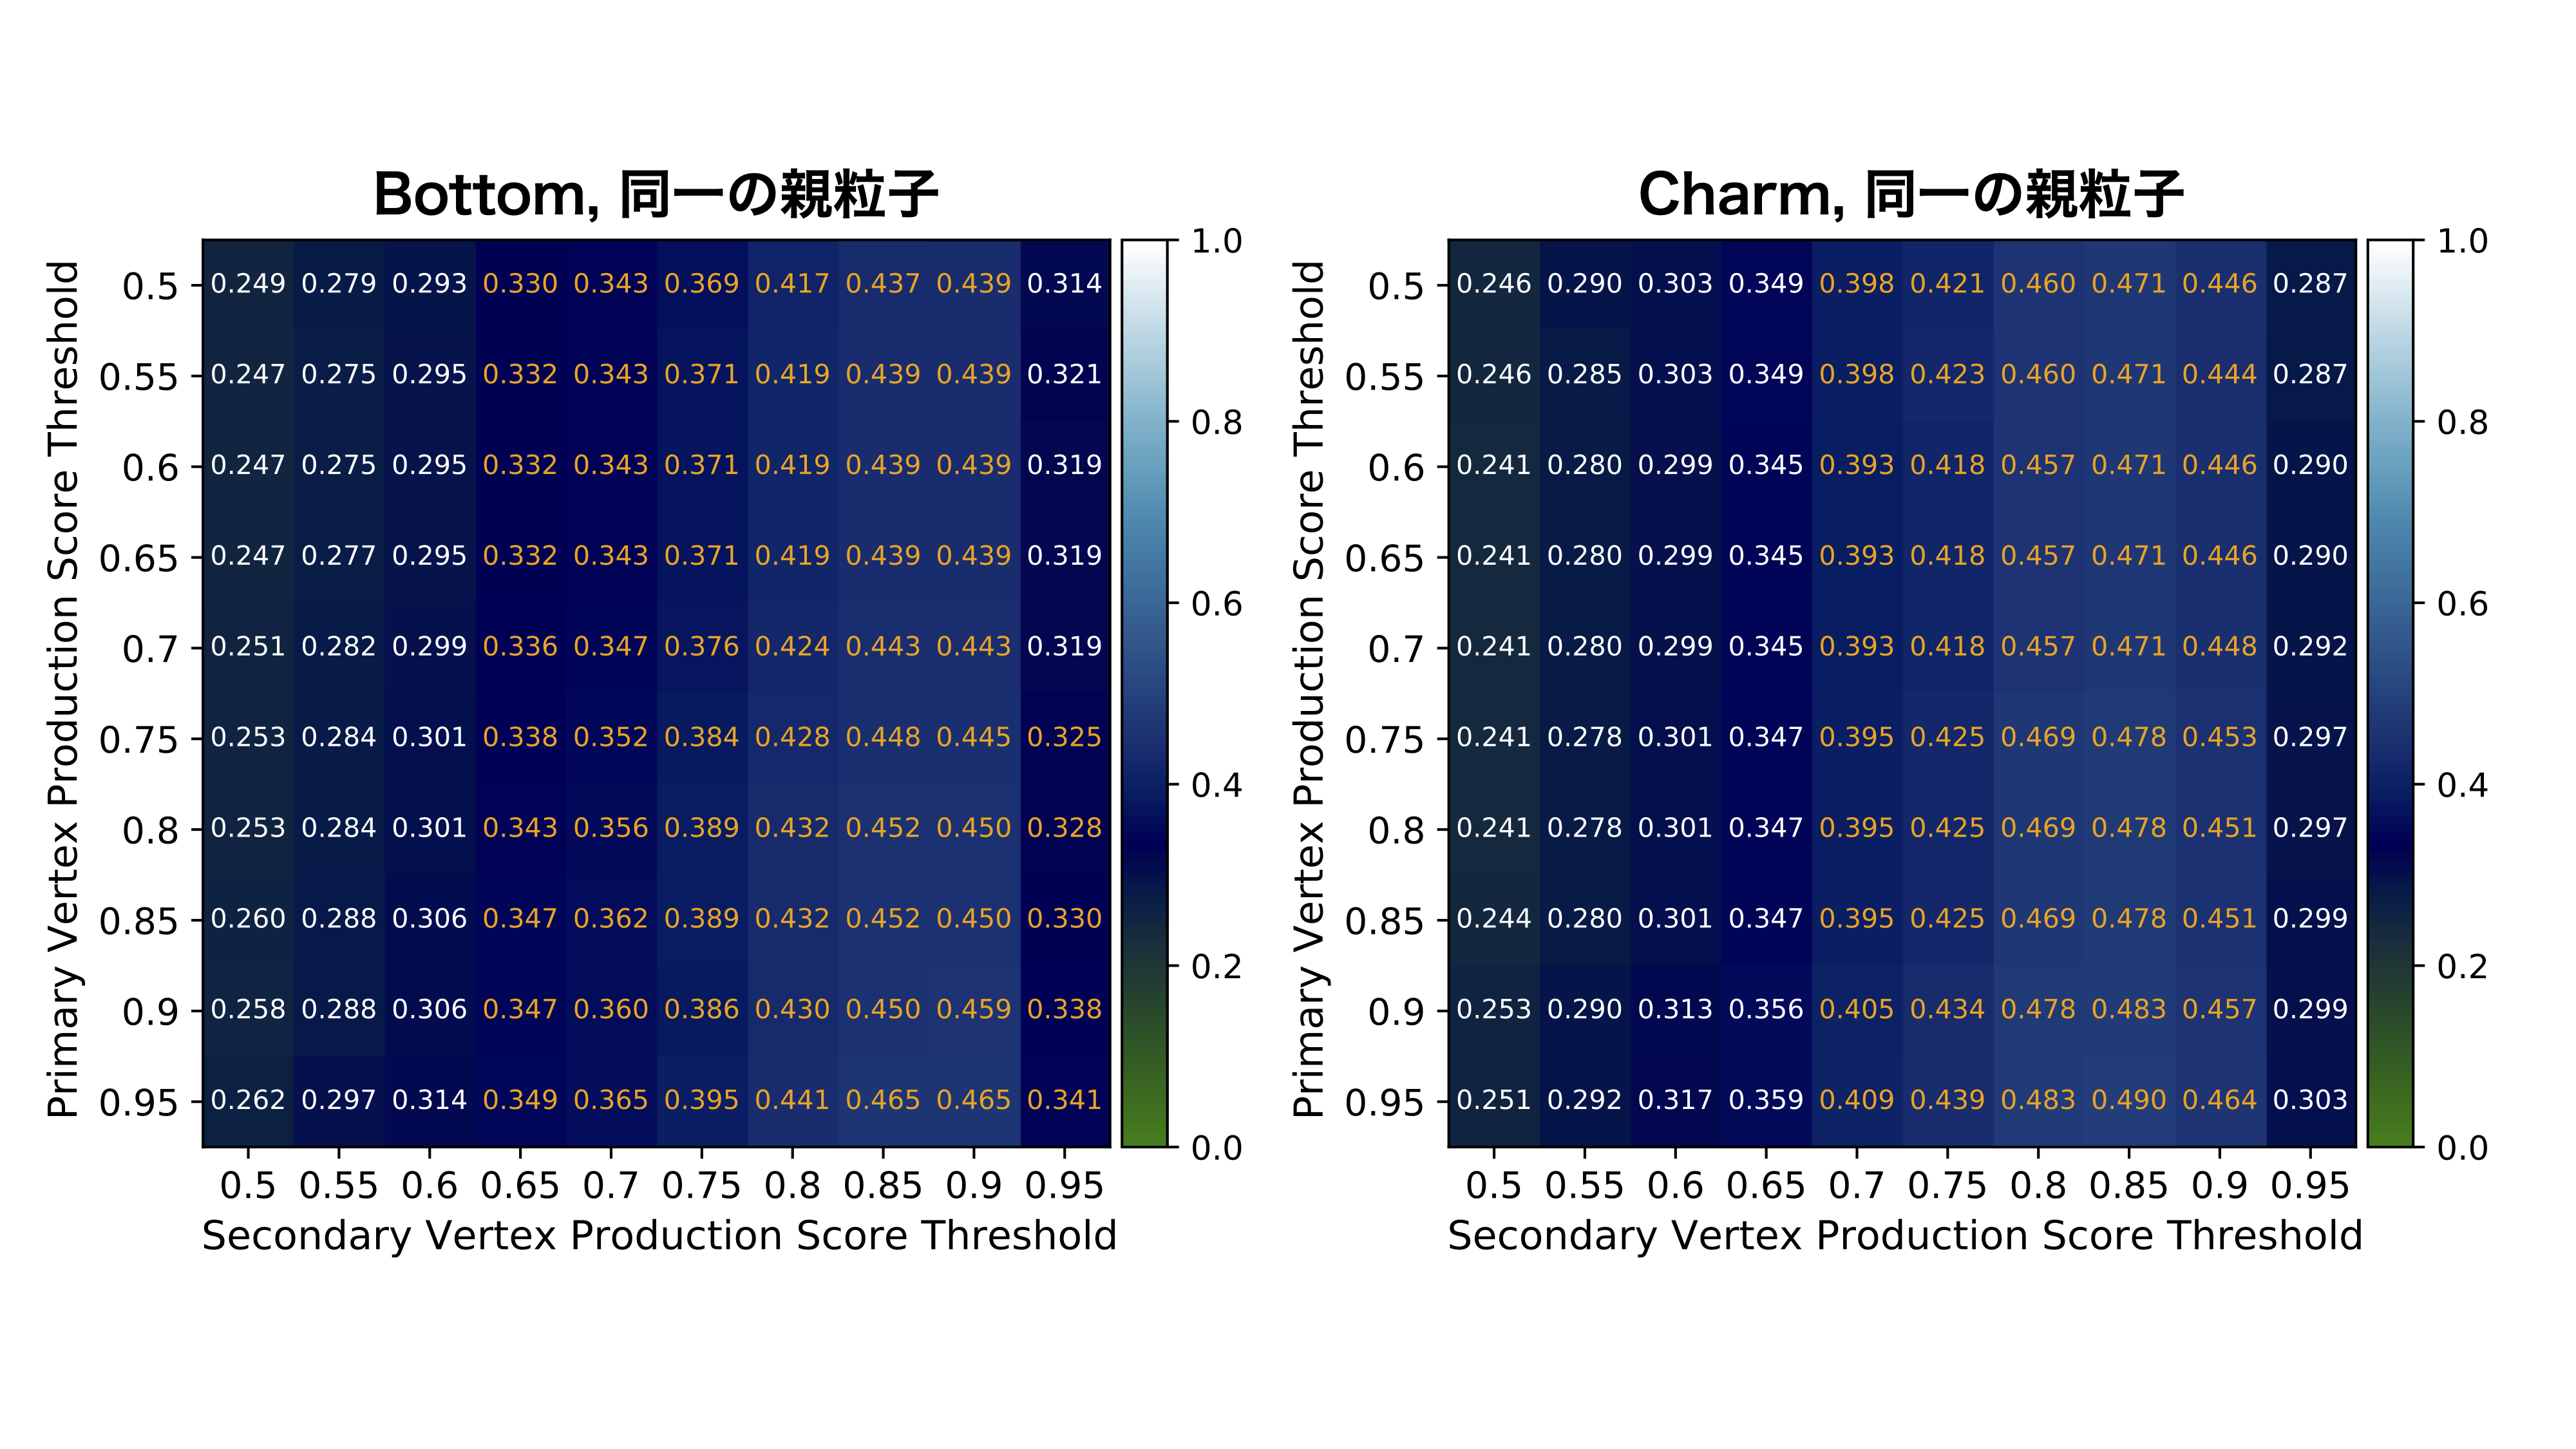
\includegraphics[trim = 0 140 0 125, width=0.9\textwidth, clip]{Figure/4VertexFinderwithDL/4-2-2-2SameParentParticle.png}
   \end{minipage} 
  \caption[閾値と崩壊点検出の性能の関係]{閾値と崩壊点検出の性能の関係。全ての図について縦軸・横軸はprimary vertex・secondary vertexのスコアの閾値である。Primary, Others, Bottom, Charmはそれぞれの飛跡がネットワークによってsecondary vertexと判断された割合を示している。同一の崩壊チェイン, 同一の親粒子は再構成されたsecondary vertex内に異なる崩壊チェインや親粒子由来の飛跡を含んでいないか評価している。}
  \label{4-2-2-2TrackEfficiency}
 %\end{tabular}
\end{figure}

ここで, 次章の評価の為, 現行の手法であるLCFIPlusの性能値より値の大きいものの数値を色付けしている。
secondary vertexの生成でのネットワークのスコアの閾値について同一の親粒子に関する性能を見ると, 閾値が大きいほど値が上昇し$0.85$付近で減少へ転じていることが分かる。
一方, BottomやCharmとその同一の崩壊チェインについての性能は閾値が大きいほど値が減少している。
したがって, 小さな閾値では一つのsecondary vertexに対して様々な飛跡が結合してしまい, 結果として, 同一の親粒子での性能が低下していると考えられる。
ただし, 同一の崩壊チェインについては常に数\%程度の差異で追従しており, 本研究のネットワークが正常に動作していることが理解できる。

PrimaryやOthersは非常に値が小さく, Primaryはprimary vertex・secondary vertexの生成でのネットワークのスコアの閾値の両方に感度を持っていることが分かる。
これはprimary vertexの生成に対して高い閾値を設けた場合, 取り逃がした真のprimary vertex由来の飛跡がsecondary vertex内に混入してしまうことを示している。
Othersについては, primary vertexの生成に対しての閾値について大きな影響を受けていない。
このことからprimary vertexは純度が高くOthersな飛跡をほとんど含んでいないと考えられる。

\newpage
%%%%%%%%%%%%%%%%%%%%%%%%%%%%%%%%%%%%%%%%%%%%%%%%%%%%%%%%%%%%%%%%%%%%%%%%%%%%%%%%%%%%%%%%%%%%%%%%%%%%%
\section{崩壊点検出の性能} \label{VFDL:SummaryofVFDL}

本章では, 現行の手法であるLCFIPlusの評価項目に則って深層学習を用いた崩壊点検出の性能を調査した。
これは次章のLCFIPlusとの比較を行う為である。

最後にデータサンプル$\rm b\bar{b}-08$での全事象を用いた性能を表\ref{PerformanceofAllEvents}に示す。
ここでは, 前節で最適化を行った閾値の値として以下の組みを使用した。
ただし, これらの性能値は\ref{chap:Comparison}章の追加のアルゴリズムを含んでいない。

\begin{itemize}
 \item SVCC・SVBB・TVCC・SVBCのスコアの和 : $0.88$
 \item 崩壊点の位置 : $30.0\ {\mathrm{mm}}$
 \item PVのタネの数 : $3$
 \item primary vertexの生成に関するスコア : $0.50$
 \item secondary vertexの生成に関するスコア : $0.75$
\end{itemize}

\begin{table}[htb]
 \centering
 \small
  \begin{tabular*}{1.0\textwidth}{@{\extracolsep{\fill}}l c c c c}\hline
    真の飛跡の種類 & Primary & Bottom & Charm & Others\\ \hline
    全飛跡の数 & 307649 & 167161 & 152314 & 86225\\
    secondary vertexと判定された飛跡の割合 & 1.2\% & 66.8\% & 74.7\% & 6.9\%\\
    ...同一の崩壊チェイン & - & 64.8\% & 69.1\% & - \\
    ...同一の親粒子 & - & 37.9\% & 40.5\% & - \\\hline
  \end{tabular*}
  \caption{データサンプル$\rm b\bar{b}-08$での全事象を用いた性能}
  \label{PerformanceofAllEvents}
\end{table}



























